\chapter{Results}\label{section:star_results}
In the following section, the  final-state charged particle distributions are compared with various  SD MC predictions, i.e. 
\begin{itemize}
	\item PYTHIA 8 4C (SaS),
	\item PYTHIA 8 A2 (MBR),
	\item PYTHIA 8 A2 (MBR-tuned): expectations obtained without arbitrary suppression of diffractive cross sections at relatively large $\xi$,
	\item HERWIG 7,
	\item EPOS LHC with combined two classes of processes: diffractive (EPOS-SD) modelled by Pomeron exchange and non-diffractive modelled by low mass excitation of the proton remnant (EPOS-SD$^\prime$).
\end{itemize}

\begin{figure}[h!]
	\centering
	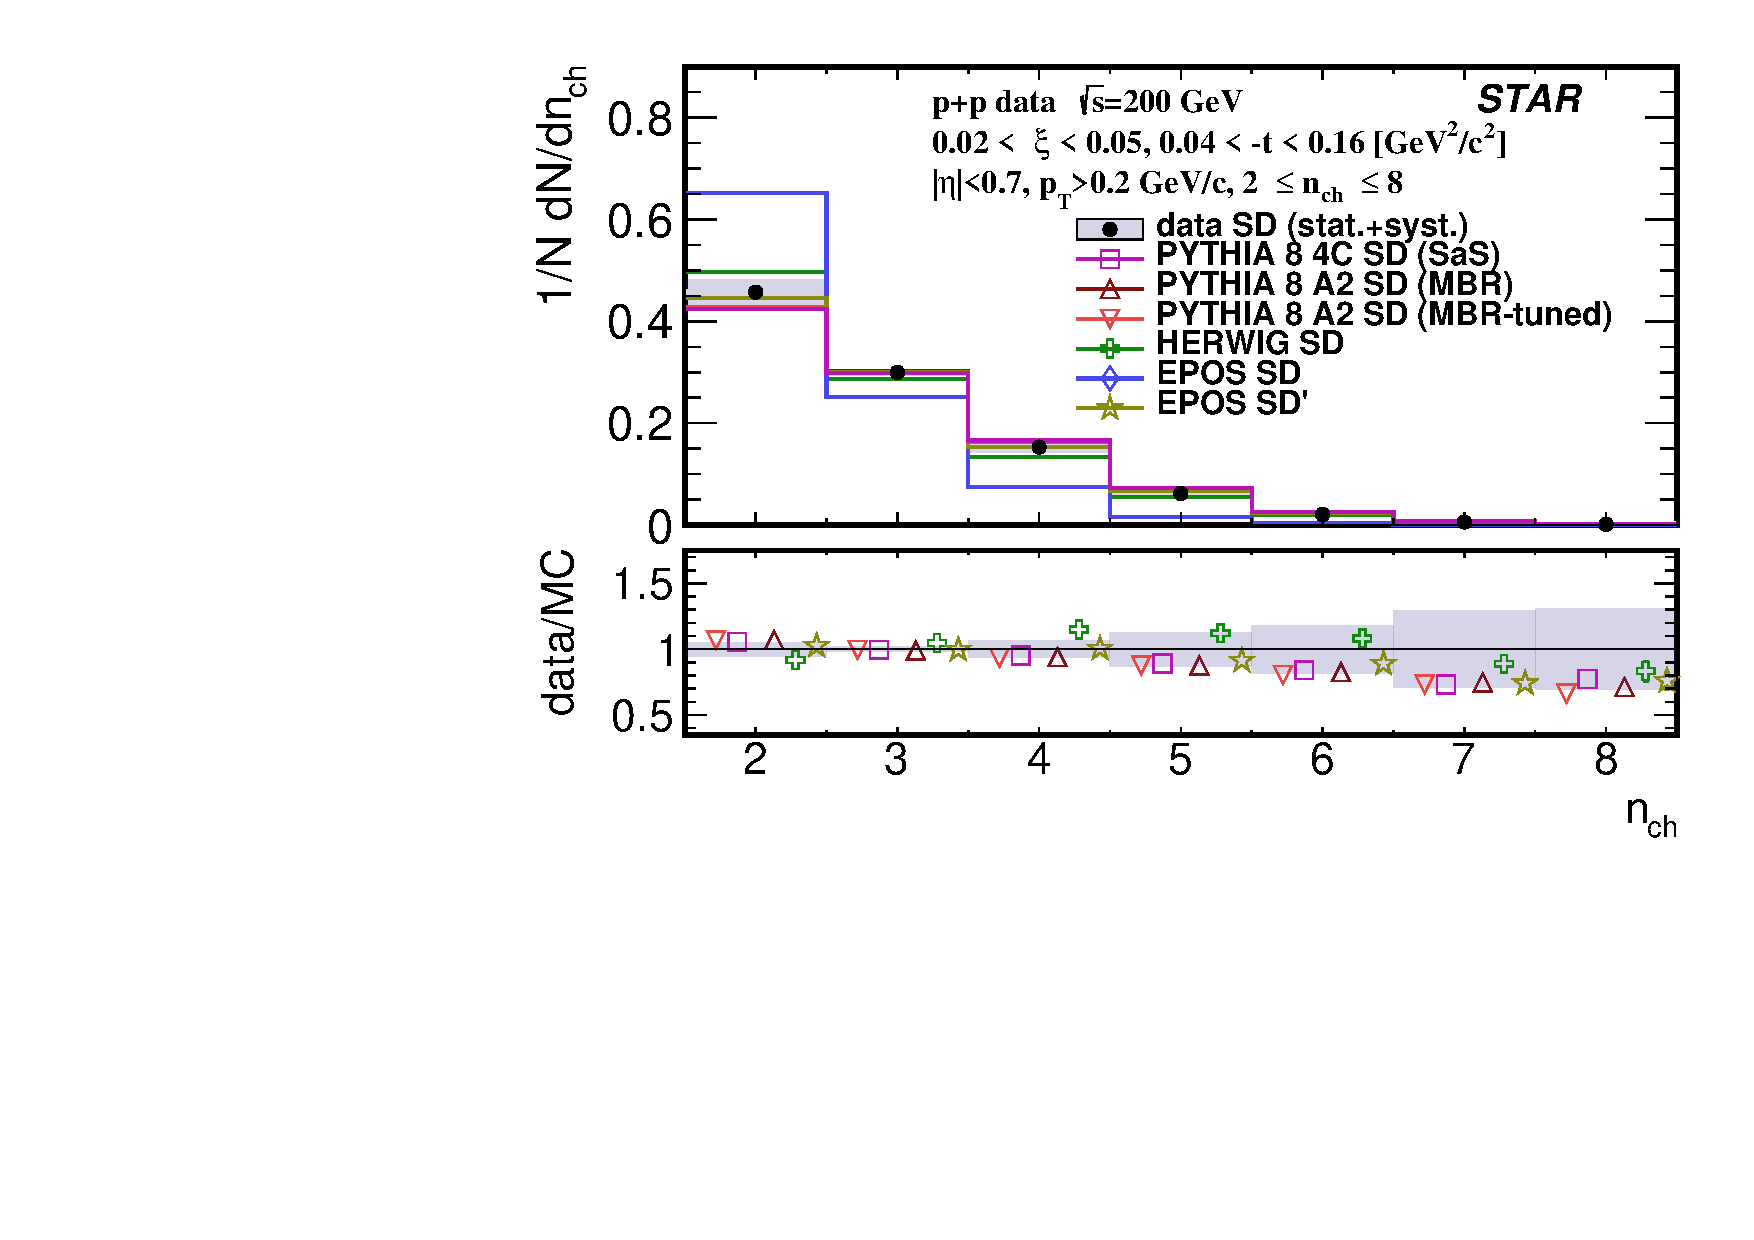
\includegraphics[width=.49\textwidth,page=1]{chapters/chrgSTAR/img/results/nch_ksi_0.pdf}
	\hfill
	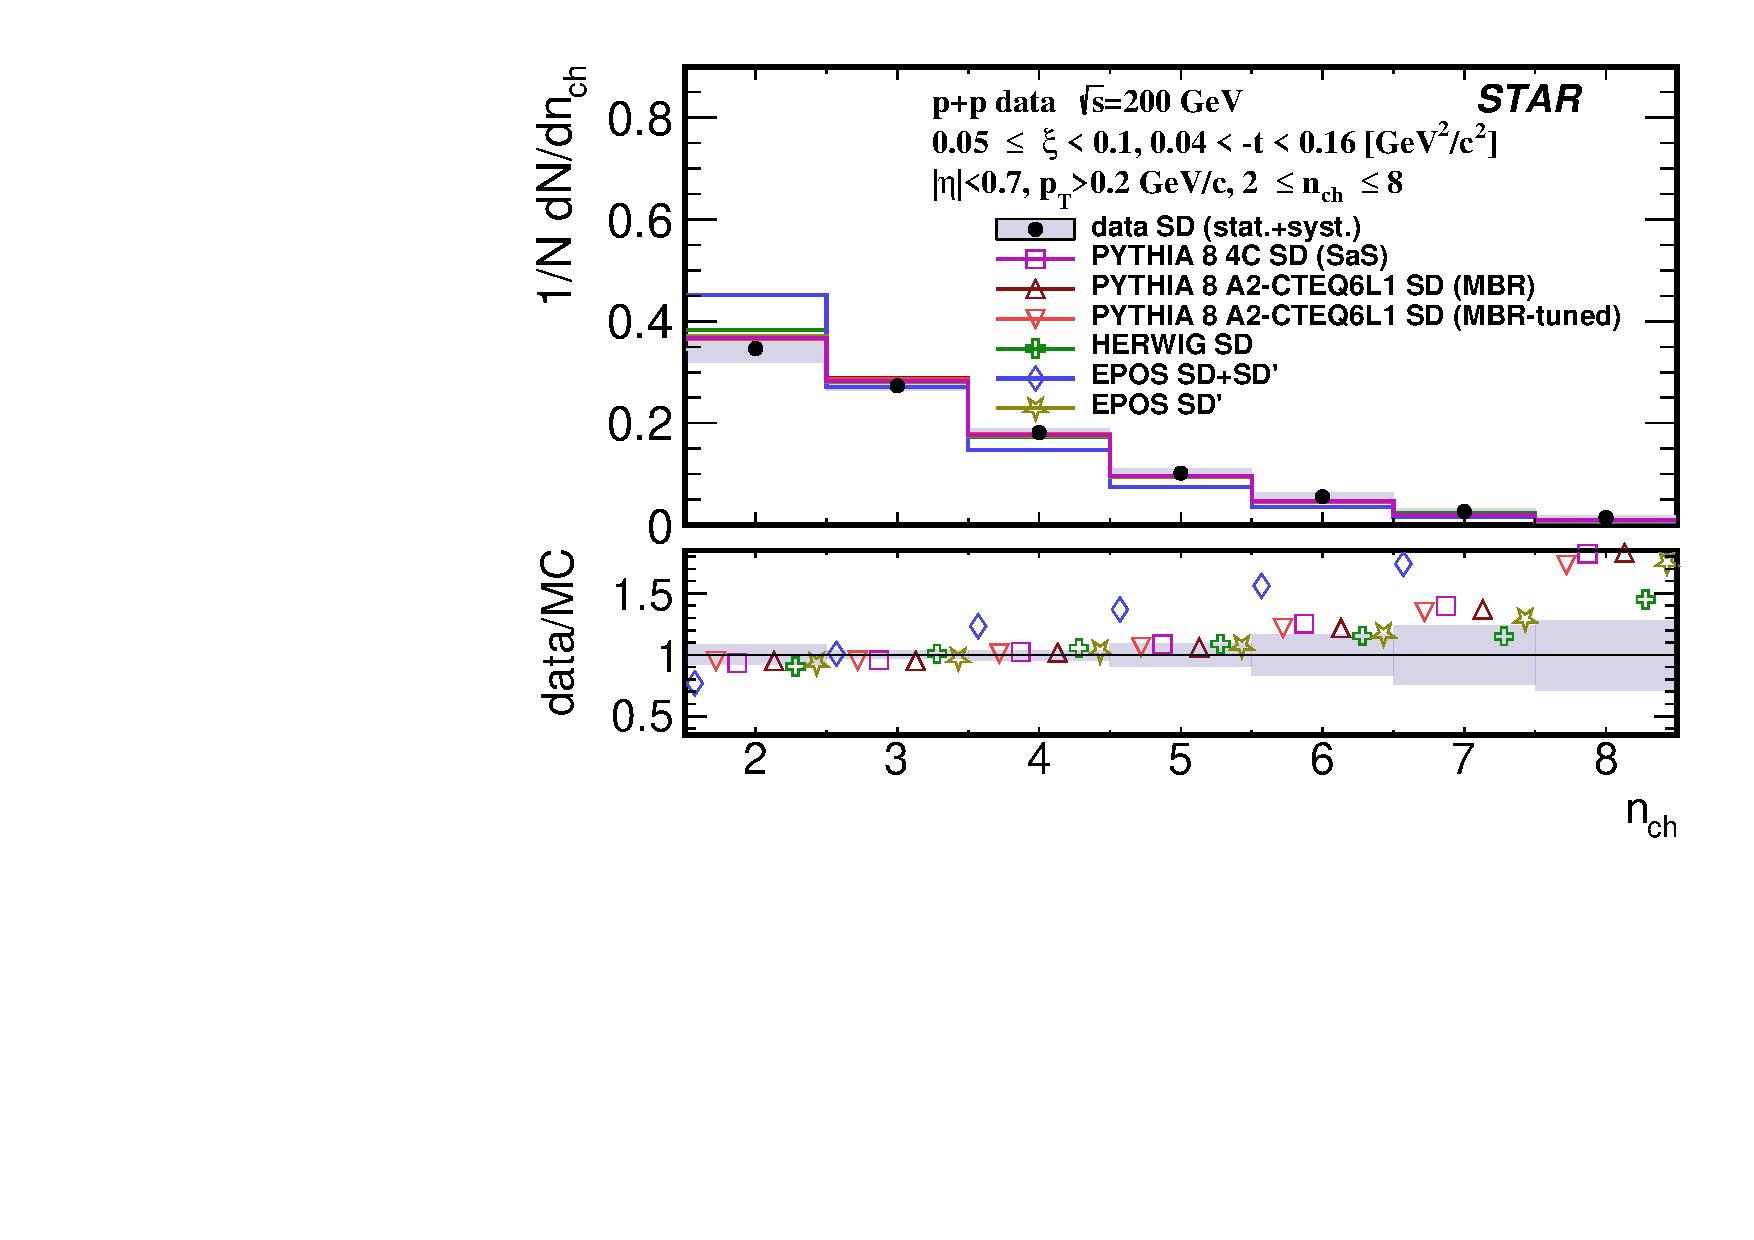
\includegraphics[width=.49\textwidth,page=1]{chapters/chrgSTAR/img/results/nch_ksi_1.pdf}
	\newline
	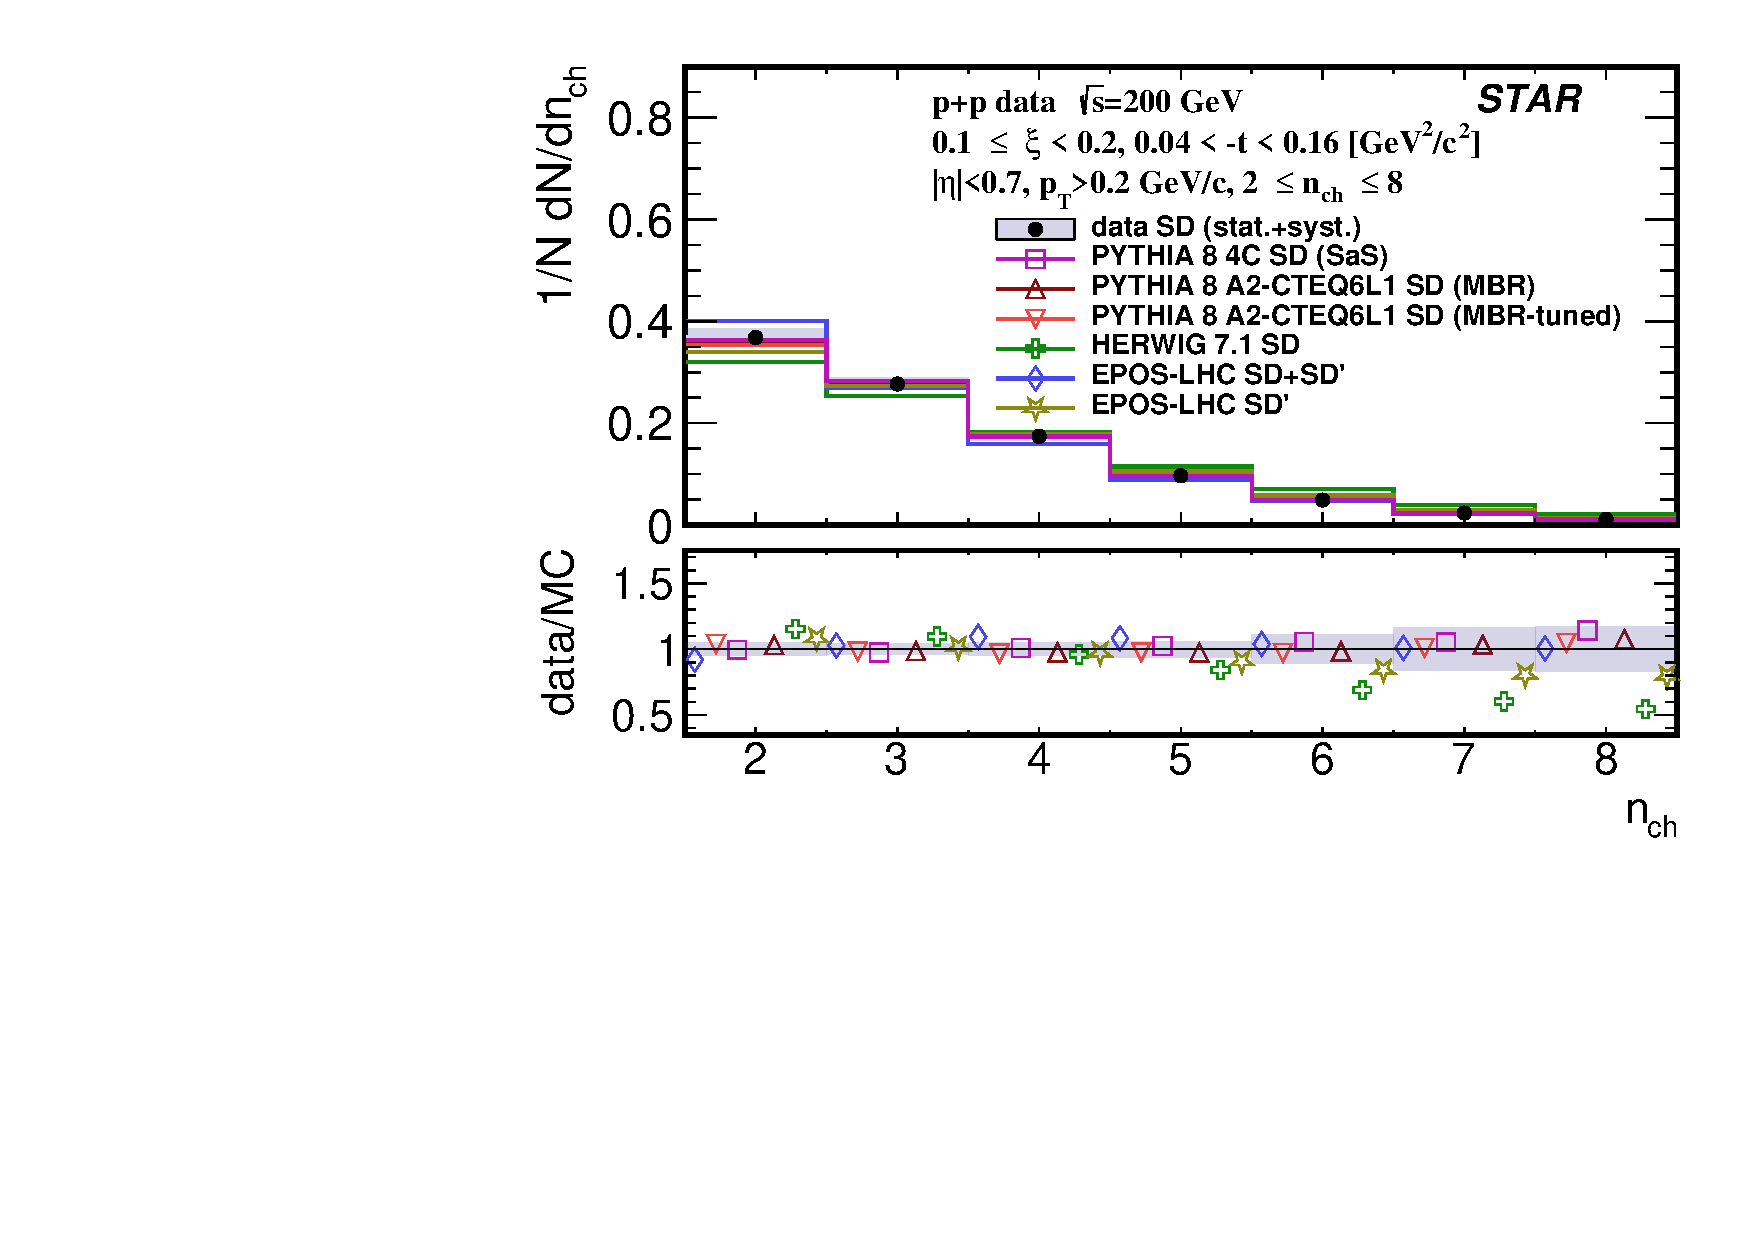
\includegraphics[width=.49\textwidth,page=1]{chapters/chrgSTAR/img/results/nch_ksi_2.pdf}
	\hfill
	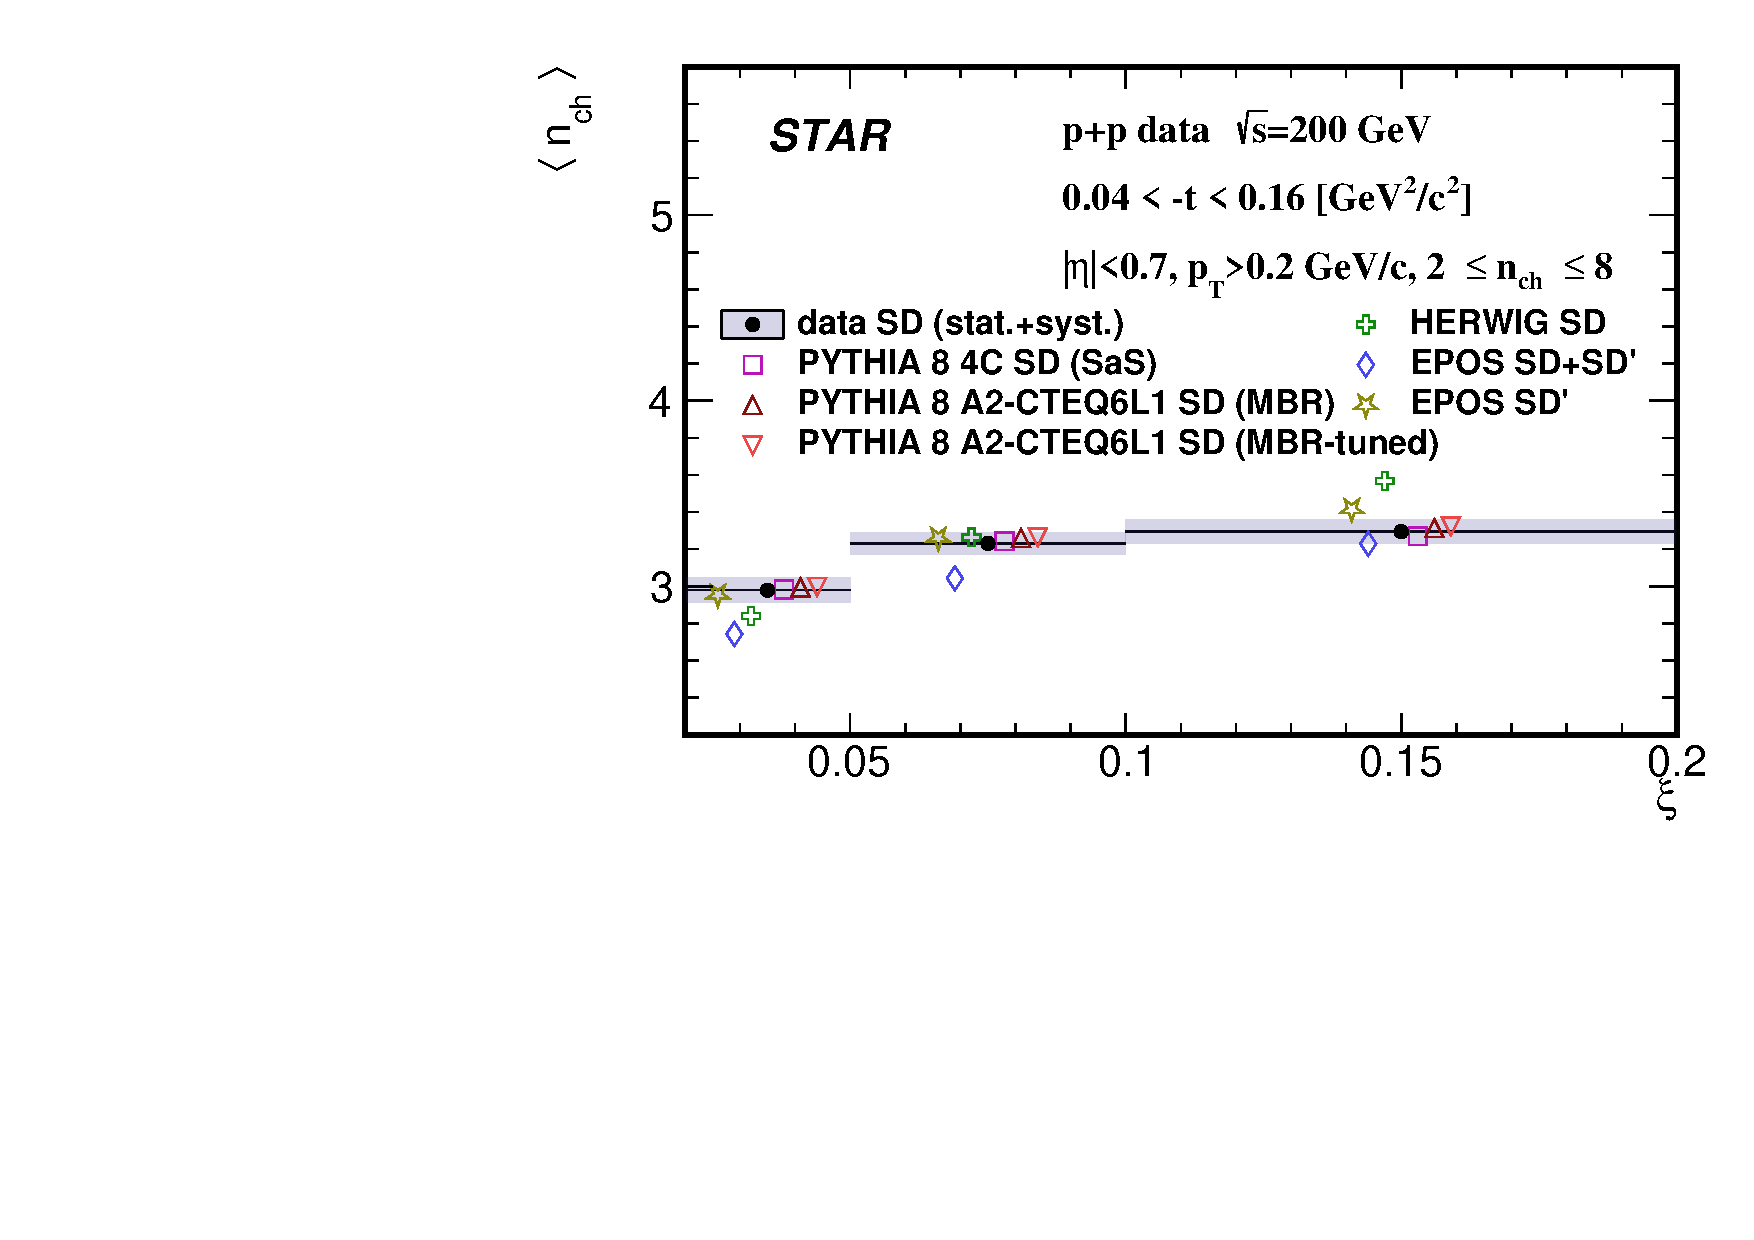
\includegraphics[width=.49\textwidth,page=1]{chapters/chrgSTAR/img/results/mean_nch_xi.pdf}
	%
	\caption{Primary charged-particle multiplicity shown separately for the~three ranges of  $\xi$: (top left) $0.02<\xi<0.05$, (top right) $0.05<\xi<0.1$, (bottom left) $0.1<\xi<0.2$ and (bottom right) the mean multiplicity $\langle n_\textrm{ch}\rangle$ as a function of $\xi$.}
	\label{fig:results_star_nch}
\end{figure}
In all figures, data are shown as solid points with error bars representing the statistical uncertainties. Gray boxes represent statistical and systematic uncertainties added in quadrature. Predictions from MC models are shown as colour histograms and markers. The~lower panel in each figure shows the ratio of data to the models' predictions. All results are presented separately for three ranges of $\xi$: $0.02 < \xi<0.05$, $0.05<\xi<0.1$, $0.1<\xi<0.2$.

Figure~\ref{fig:results_star_nch} shows primary charged-particle multiplicity  separately for the~three ranges of $\xi$ and the mean multiplicity $\langle n_\textrm{ch}\rangle$ as a function of $\xi$.  Data follow the~expected increase of  $\langle n_\textrm{ch}\rangle$ with $\xi$ due to the larger diffractive masses probed by increasing $\xi$ in SD process. The shapes of the measured distributions are reproduced reasonably well by all models except EPOS SD+SD$^\prime$ which predicts  smaller $\langle n_\textrm{ch}\rangle$  for $0.02<\xi<0.1$  and HERWIG-SD which for $0.1<\xi<0.2$ predicts too large $\langle n_\textrm{ch}\rangle$.
\begin{figure}[h!]
	\centering
	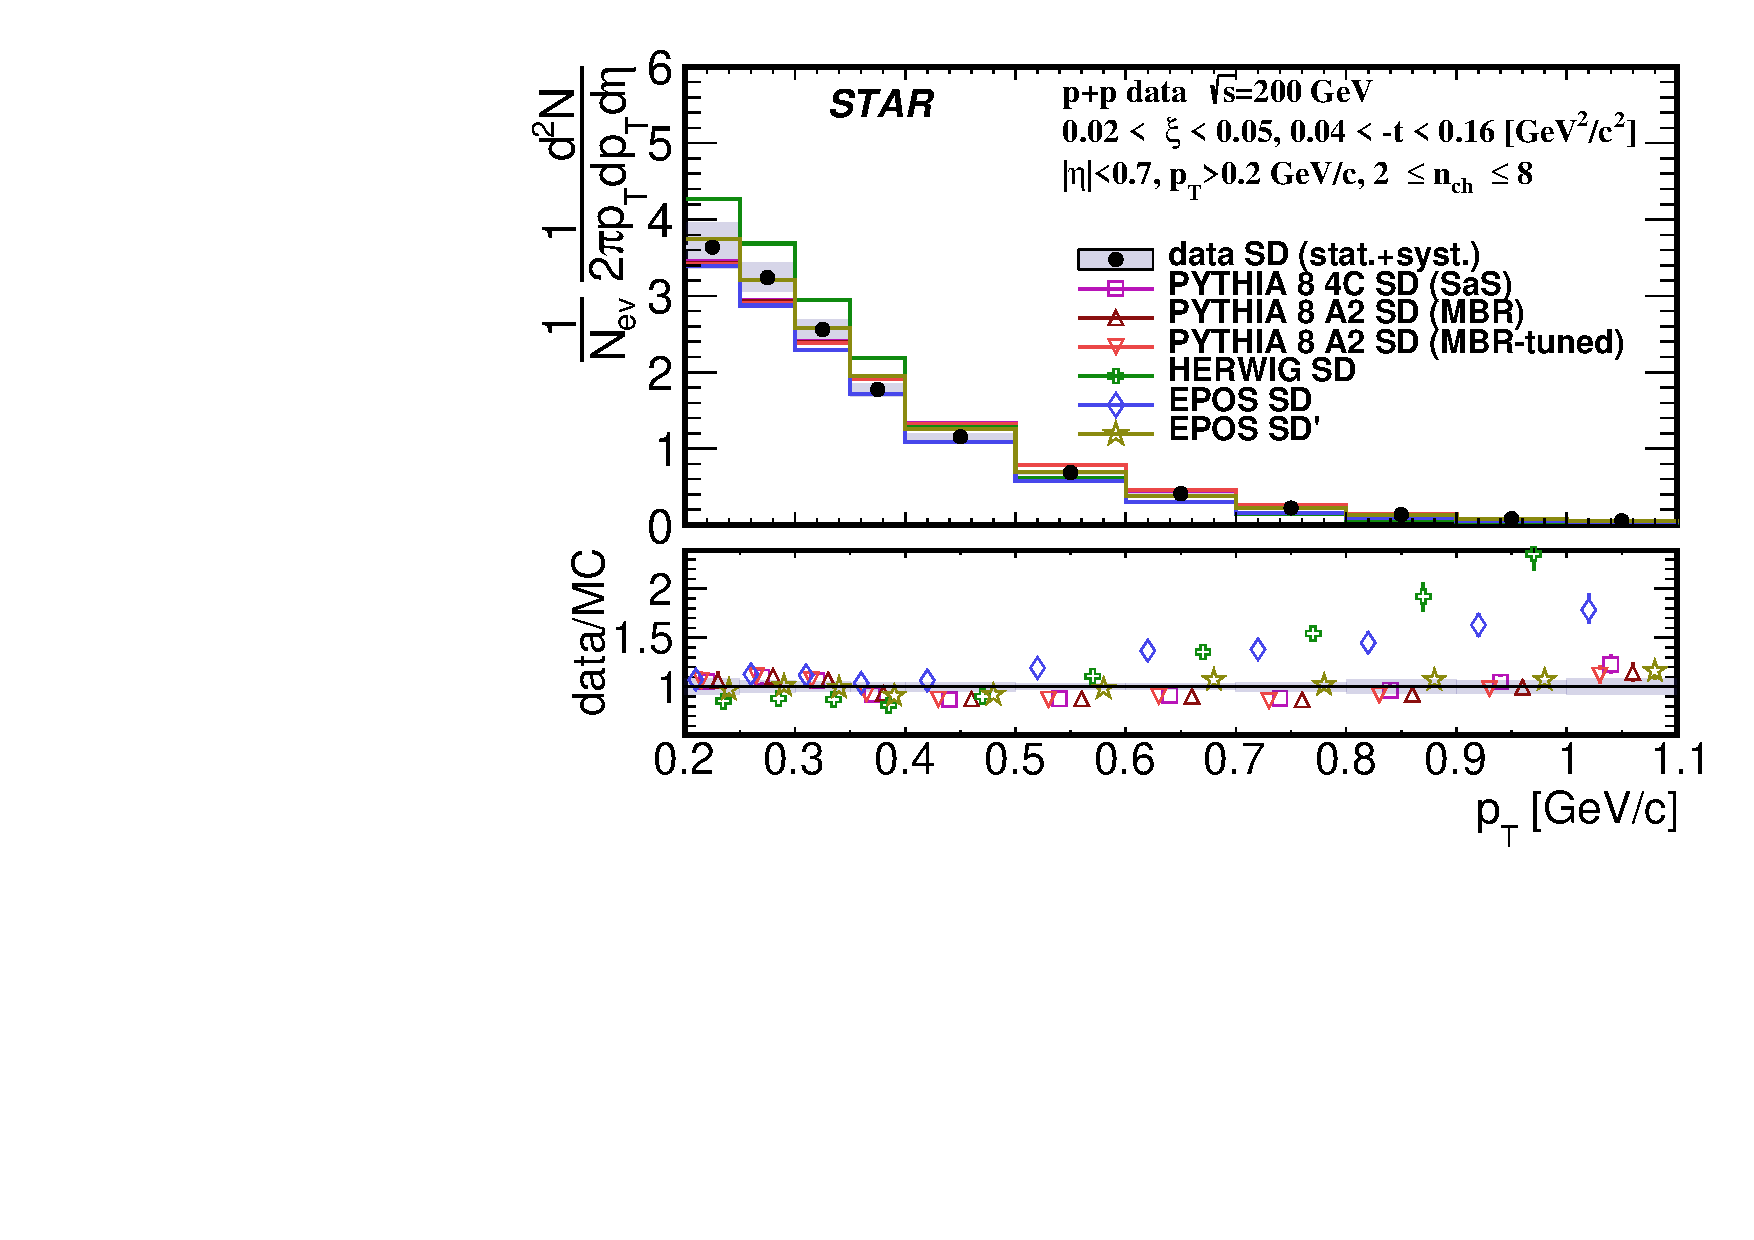
\includegraphics[width=.49\textwidth,page=1]{chapters/chrgSTAR/img/results/out_pt_ksi_0.pdf}
	\hfill
	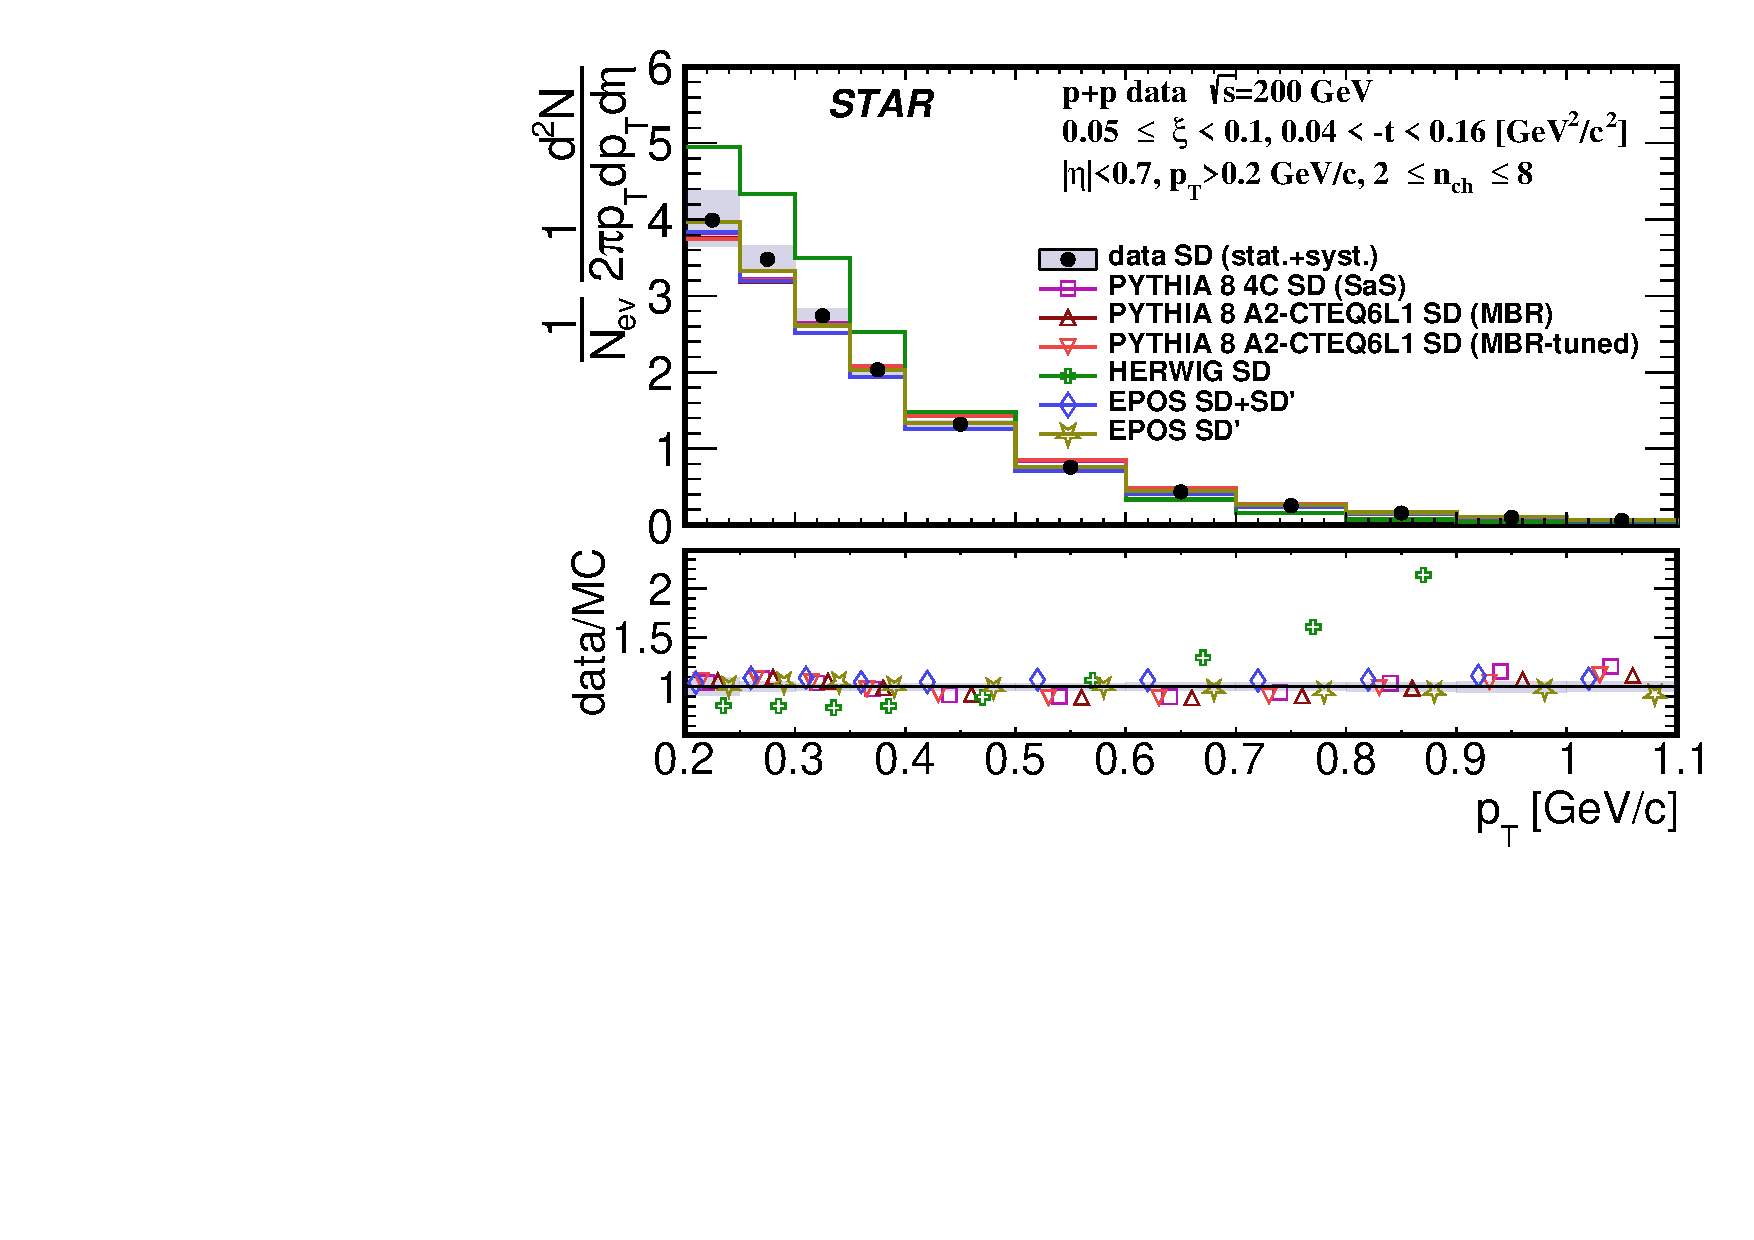
\includegraphics[width=.49\textwidth,page=1]{chapters/chrgSTAR/img/results/out_pt_ksi_1.pdf}
	\newline
	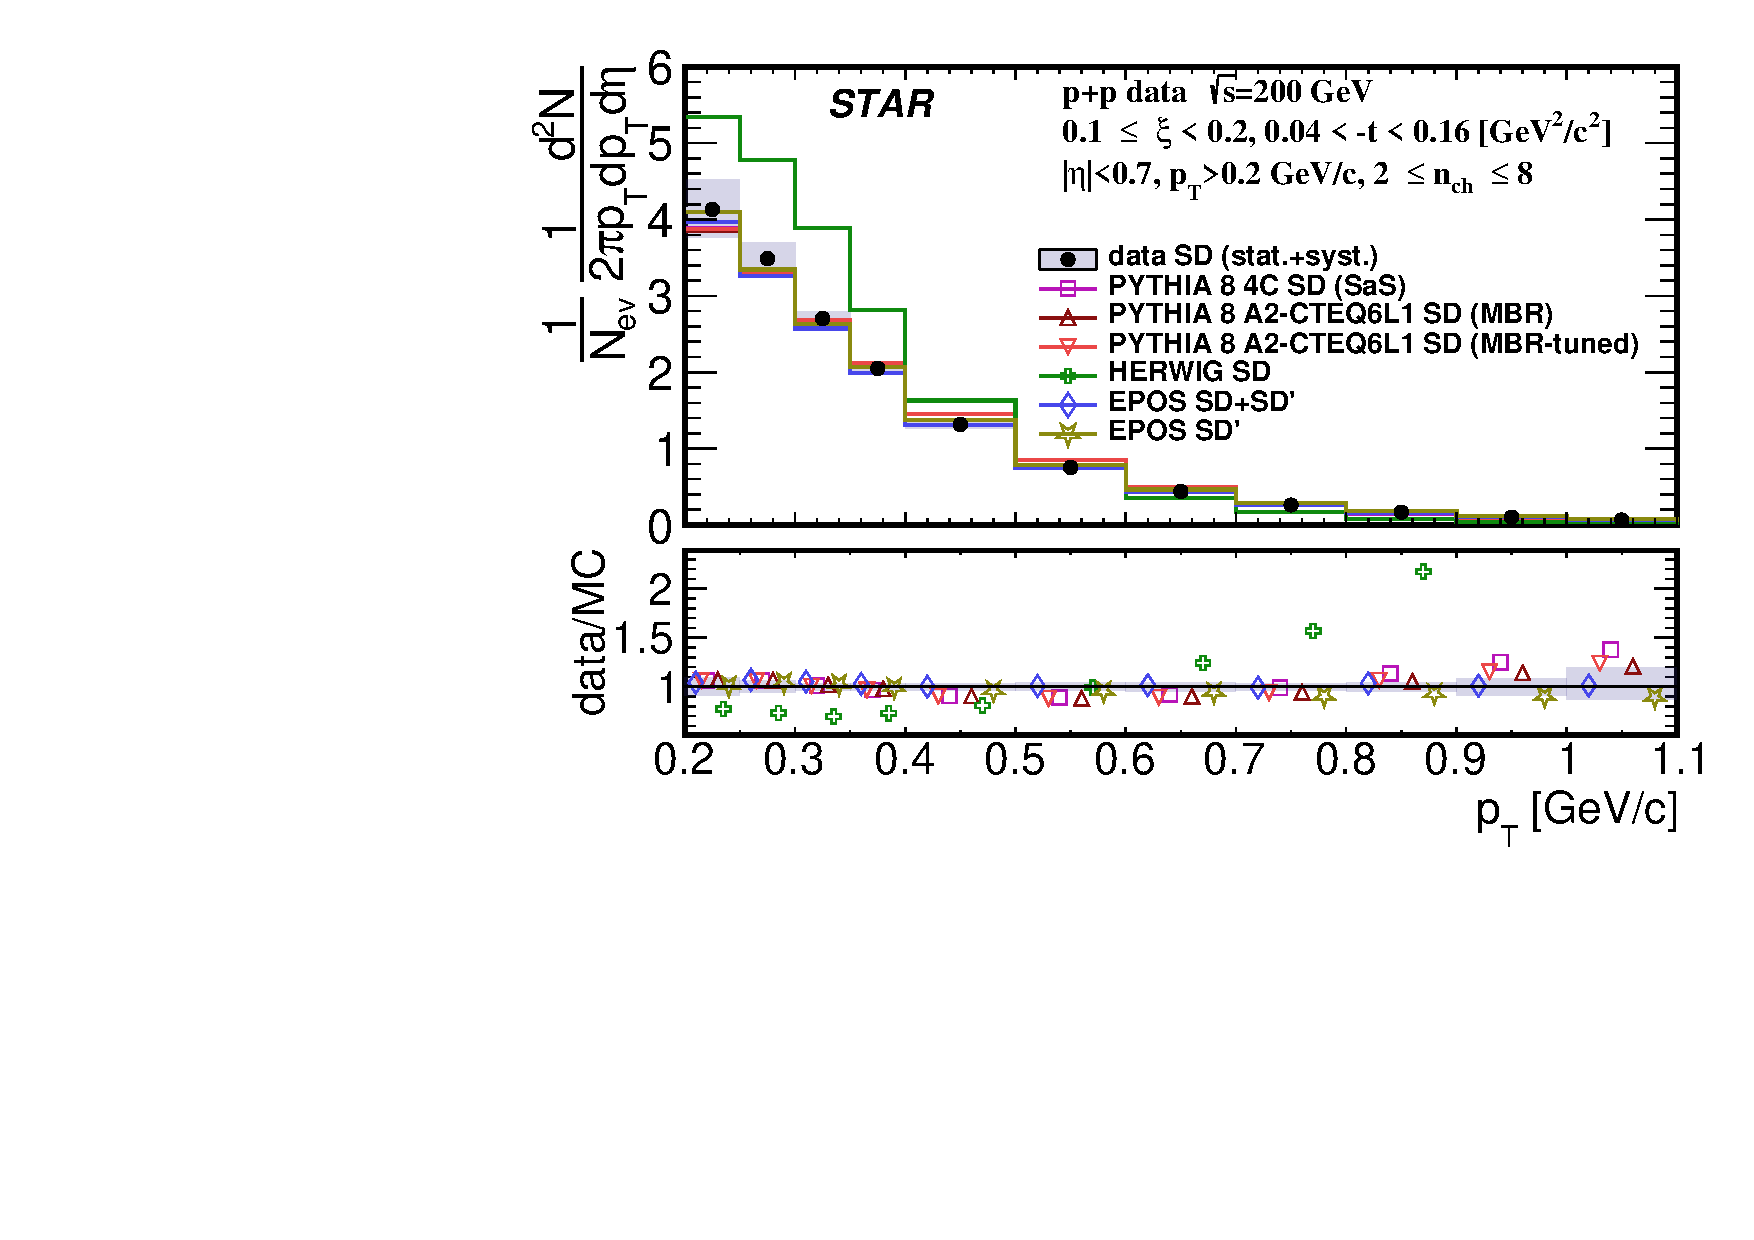
\includegraphics[width=.49\textwidth,page=1]{chapters/chrgSTAR/img/results/out_pt_ksi_2.pdf}
	\hfill
	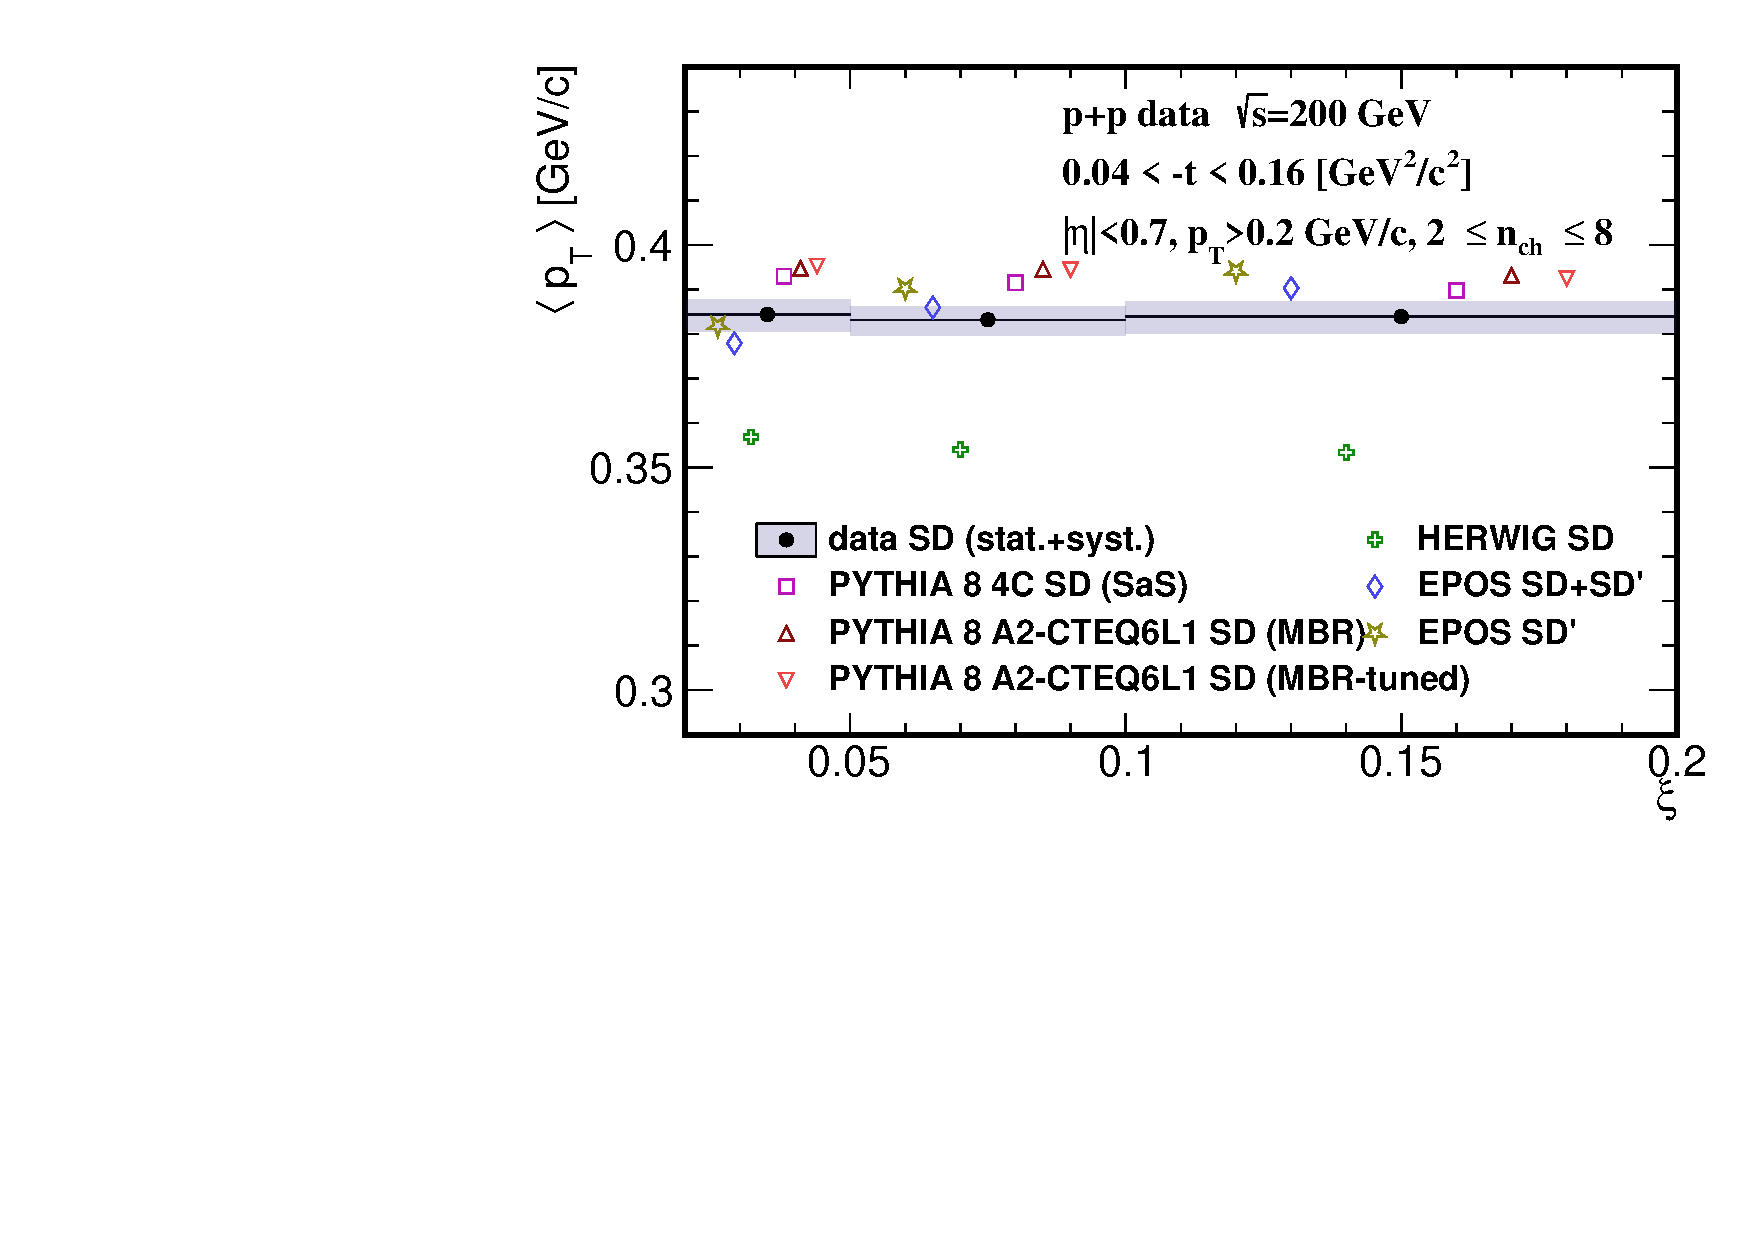
\includegraphics[width=.49\textwidth,page=1]{chapters/chrgSTAR/img/results/mean_pt_xi.pdf}
	%
	\caption{Primary charged-particle multiplicities as a function of $p_\textrm{T}$ shown separately for the~three ranges of  $\xi$: (top left) $0.02<\xi<0.05$, (top right) $0.05<\xi<0.1$, (bottom left) $0.1<\xi<0.2$ and (bottom right) the mean transverse momentum $\langle p_\textrm{T}\rangle$ as a function of $\xi$.}
	\label{fig:results_star_pt}
\end{figure}

Figure~\ref{fig:results_star_pt} shows primary charged-particle multiplicities as a function of $p_\textrm{T}$  separately for the~three ranges of $\xi$ and the mean transverse momentum $\langle p_\textrm{T}\rangle$ as a function of $\xi$. Data show that $\langle p_\textrm{T}\rangle$ depends very weakly on $\xi$. Models describe data fairly well except HERWIG-SD which predicts much steeper dependence of particle density with $p_\textrm{T}$ in all three $\xi$ ranges. %and EPOS-SD which significantly underestimates particle density especially at large $p_\textrm{T}$.
\begin{figure}[h!]
	\centering
	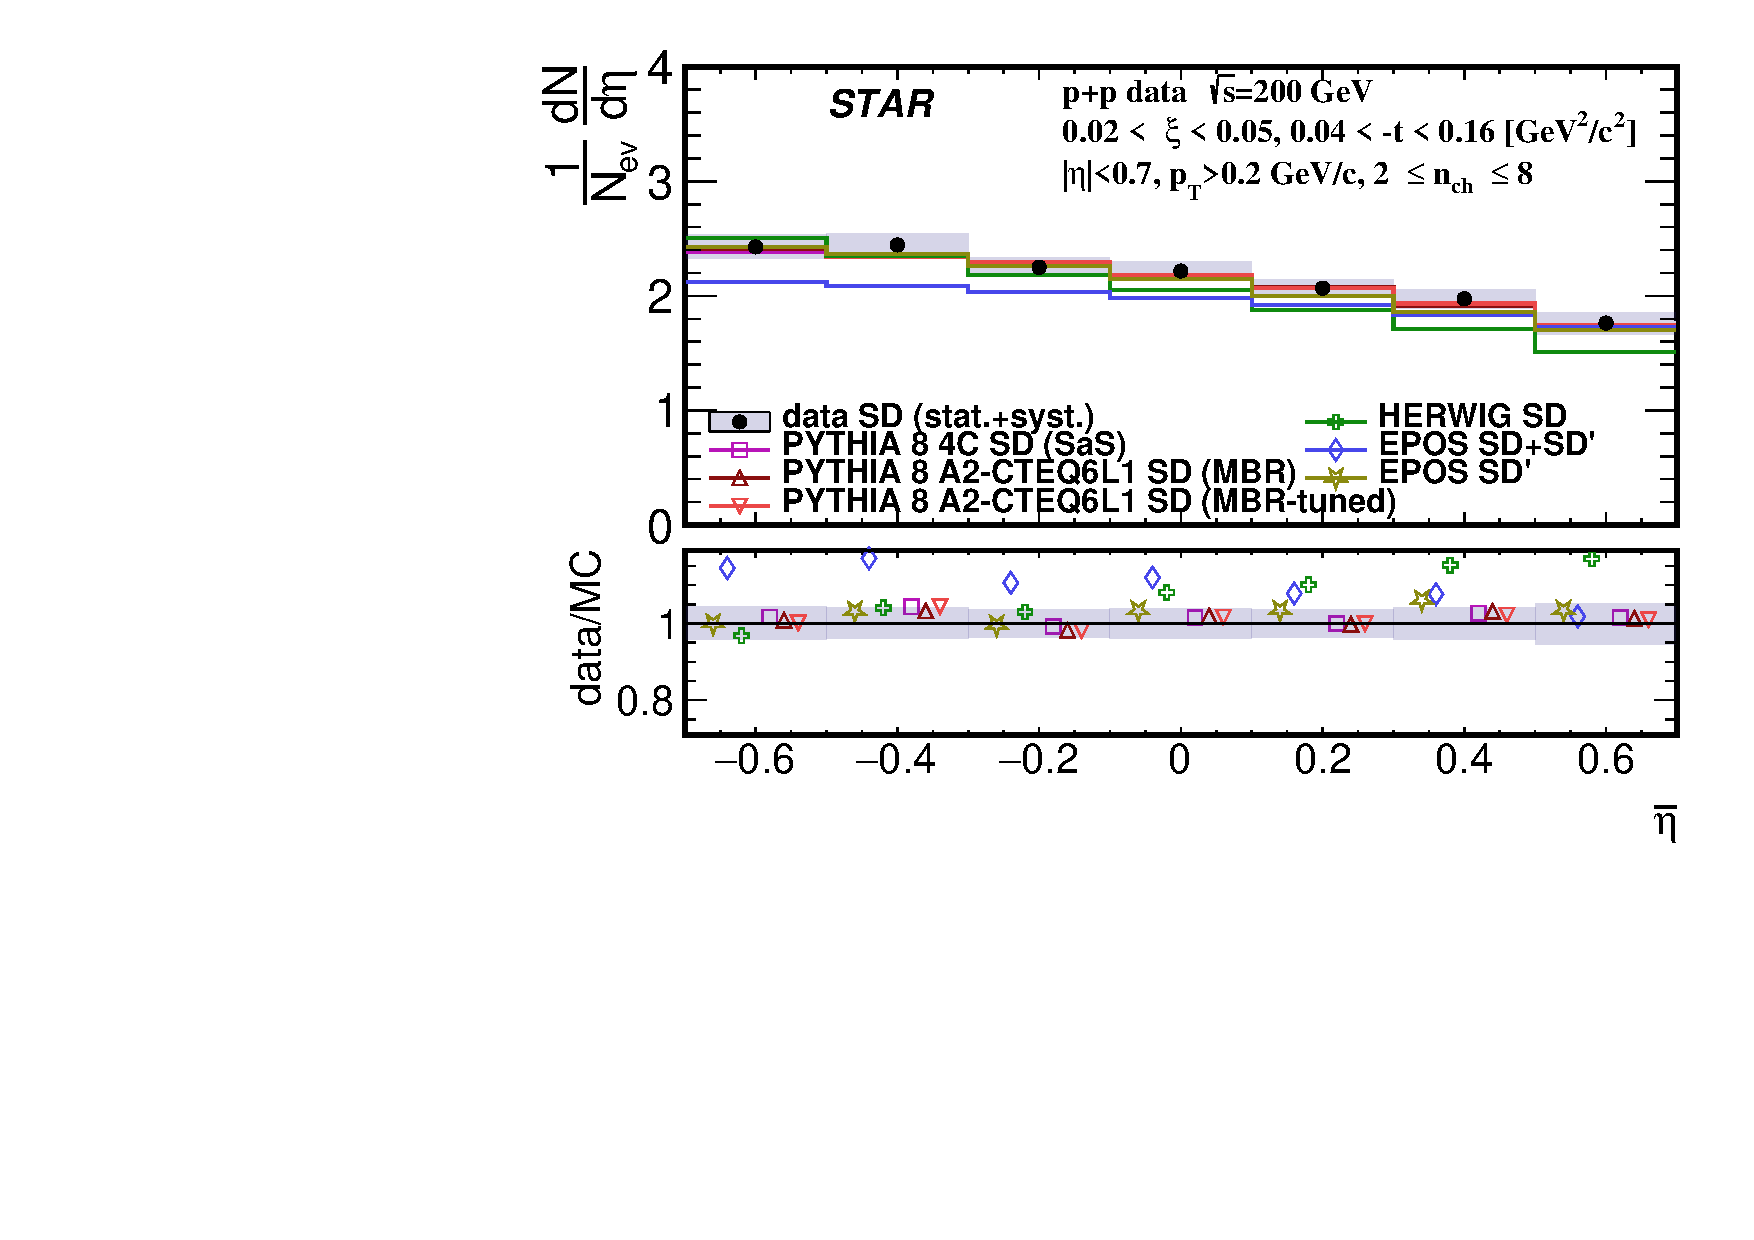
\includegraphics[width=.49\textwidth,page=1]{chapters/chrgSTAR/img/results/out_eta_SD_0.pdf}
	\hfill
	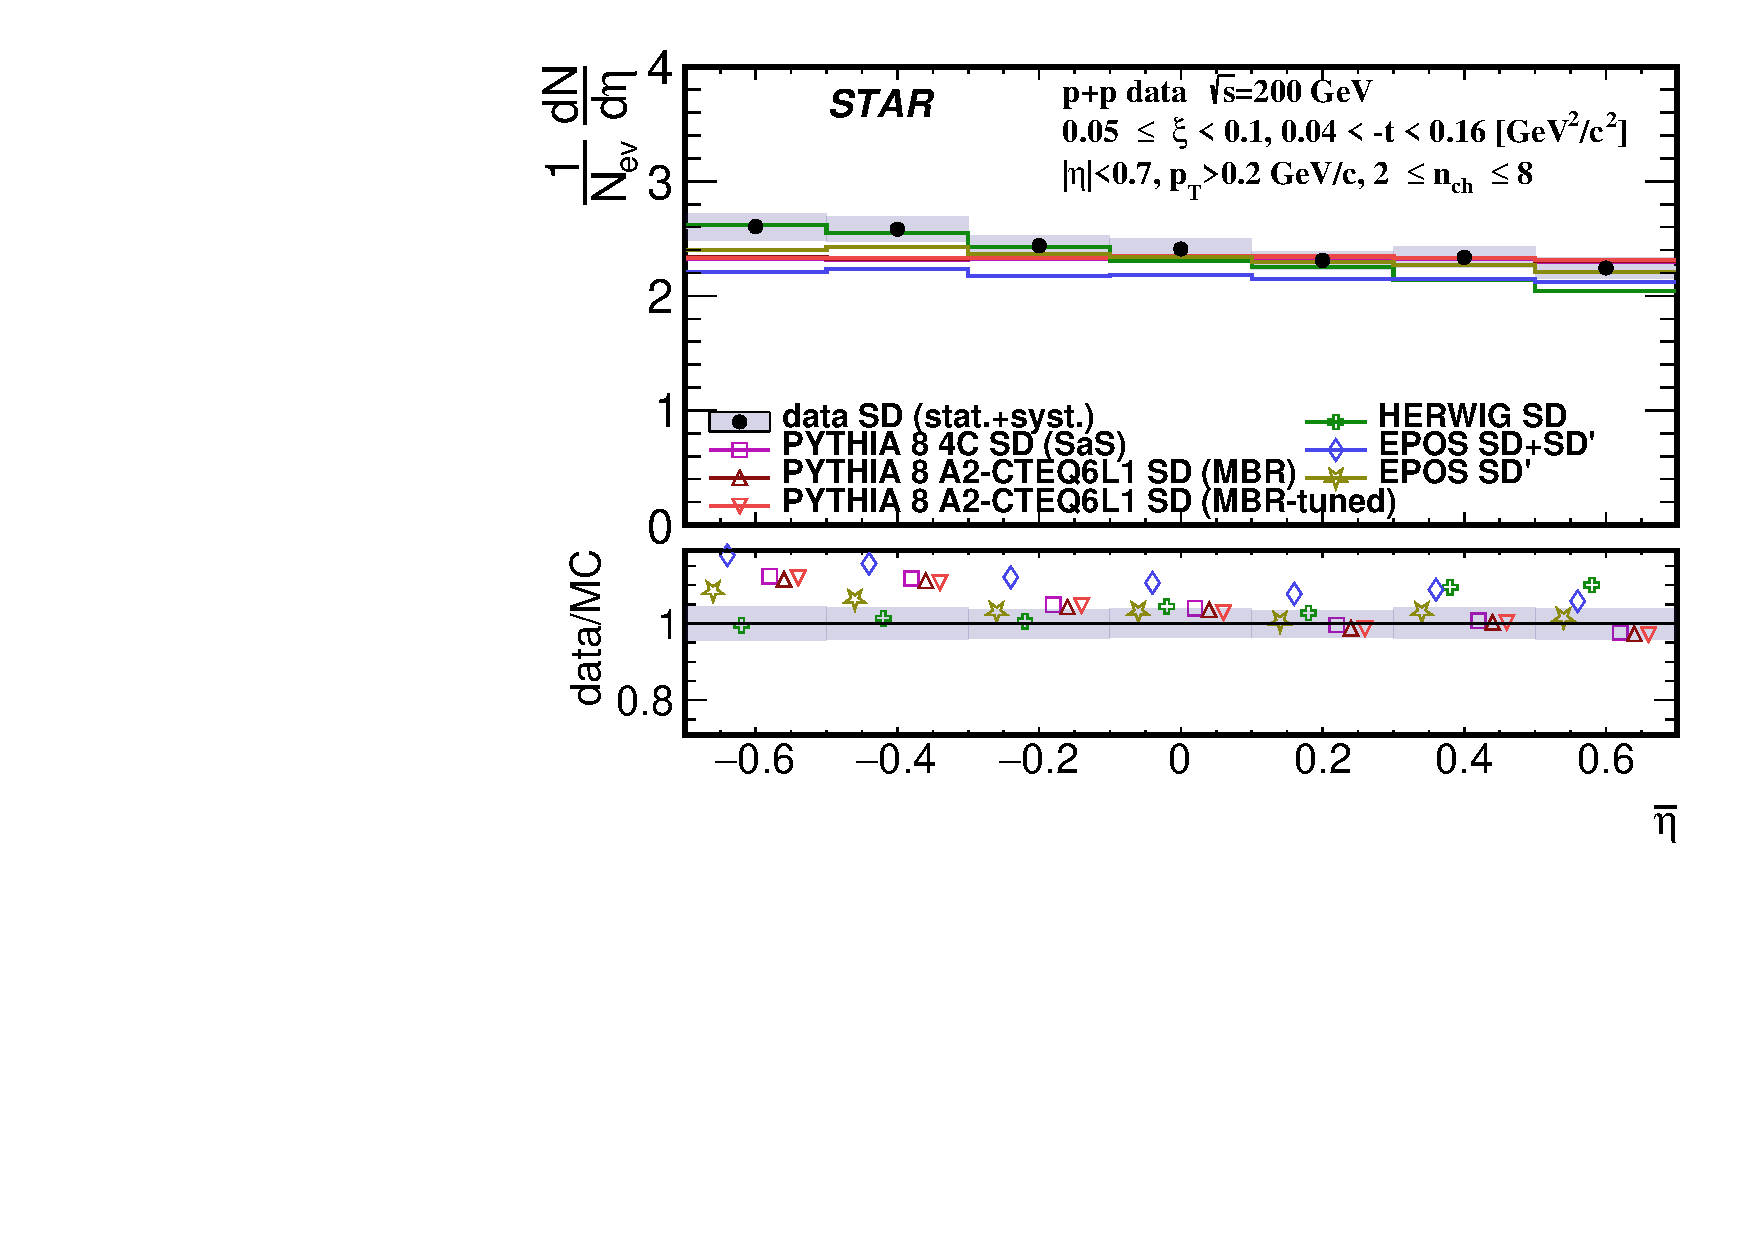
\includegraphics[width=.49\textwidth,page=1]{chapters/chrgSTAR/img/results/out_eta_SD_1.pdf}
	\newline
	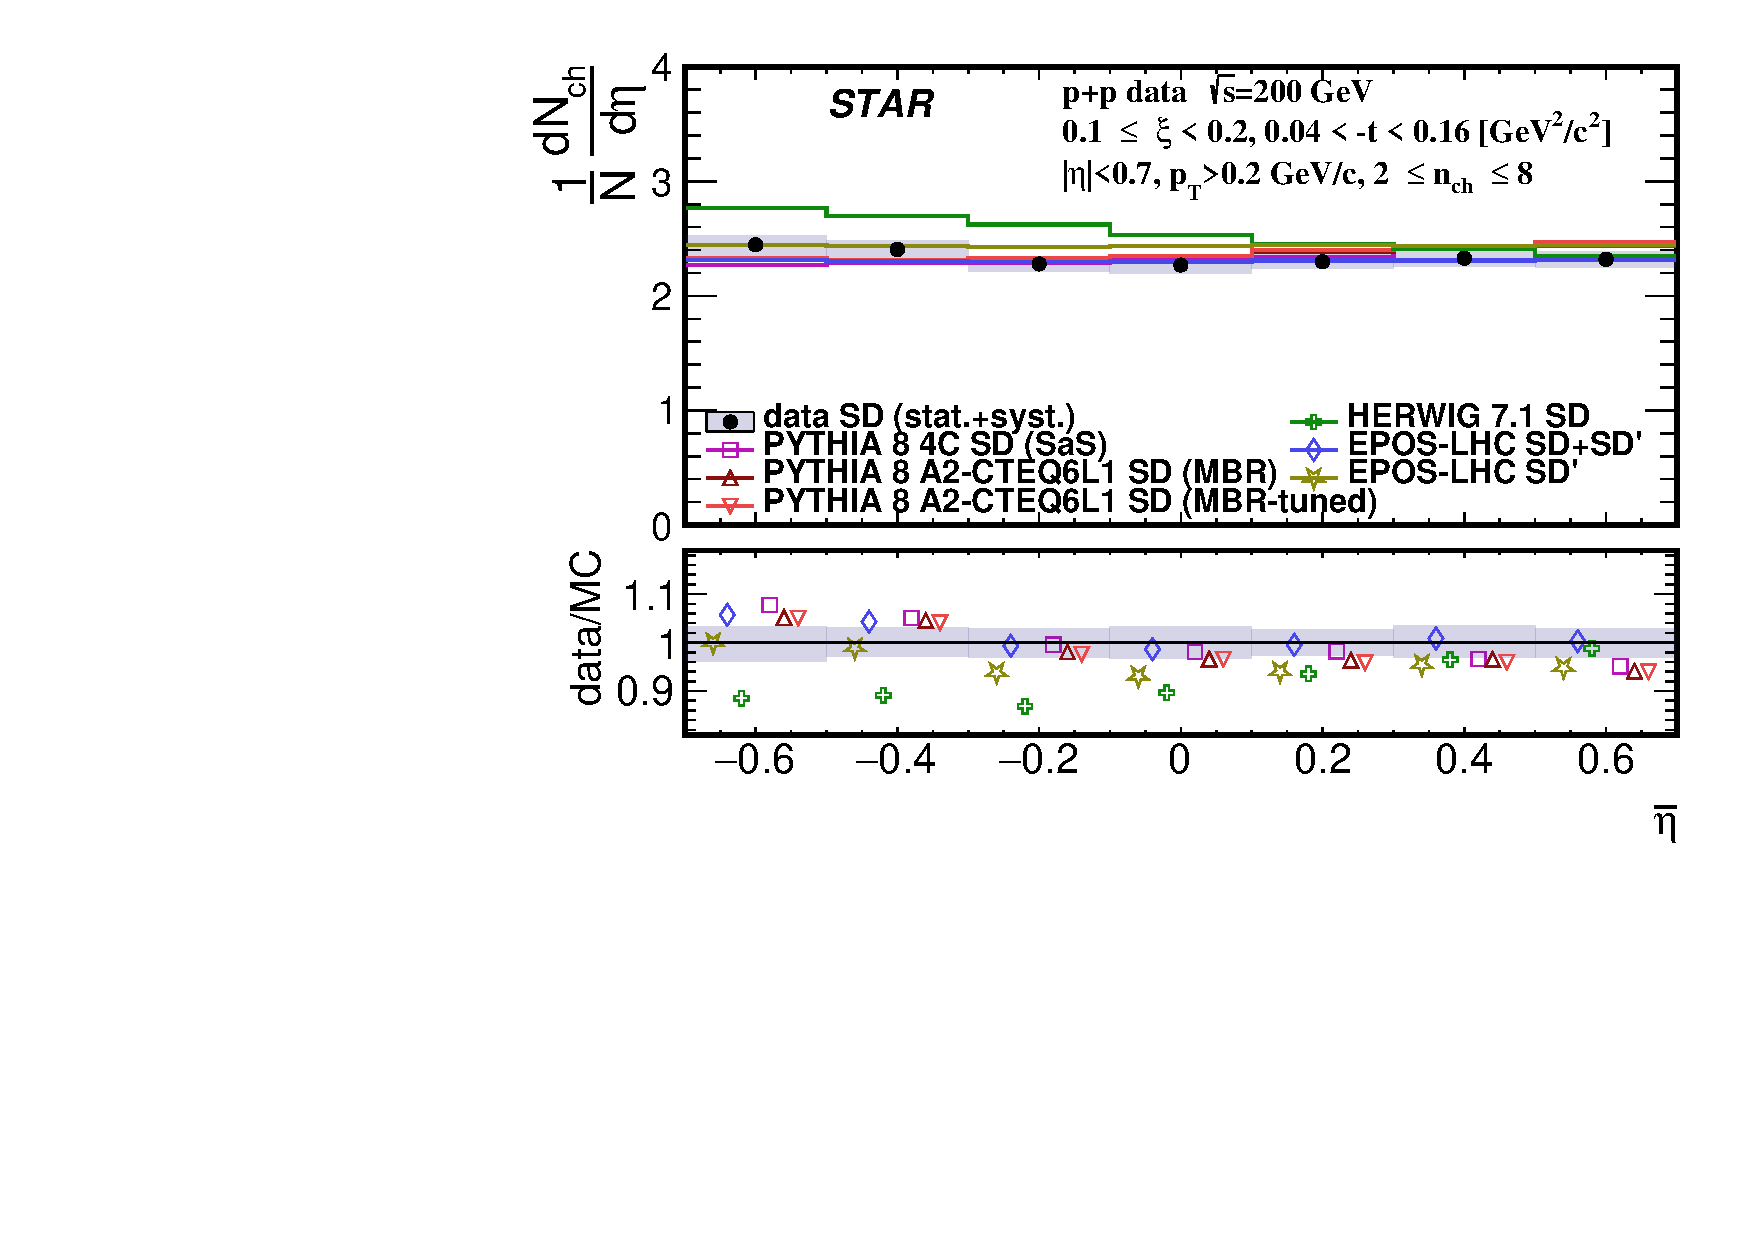
\includegraphics[width=.49\textwidth,page=1]{chapters/chrgSTAR/img/results/out_eta_SD_2.pdf}
	\hfill
	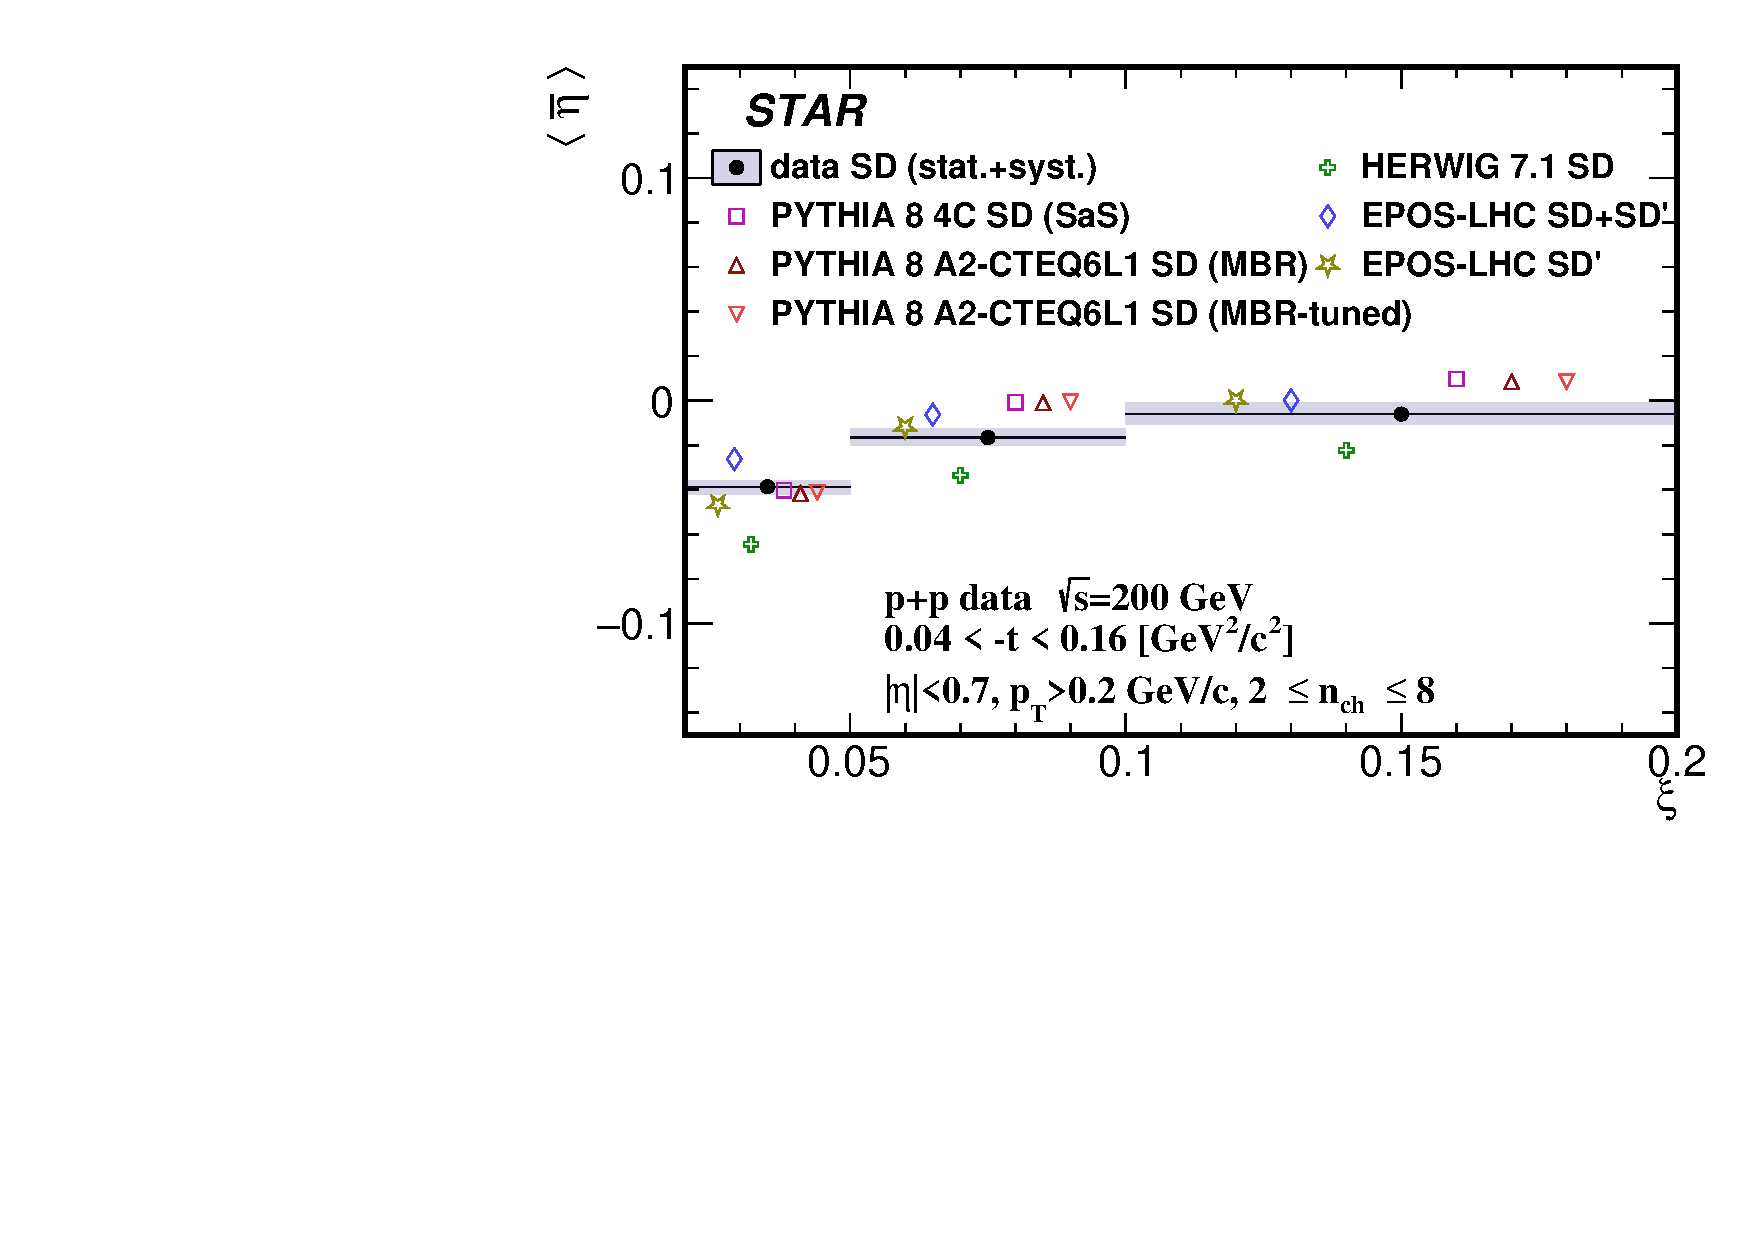
\includegraphics[width=.49\textwidth,page=1]{chapters/chrgSTAR/img/results/mean_eta_xi.pdf}
	%
	\caption{Primary charged-particle multiplicity as a function of $\bar{\eta}$ shown  separately for the~three ranges of  $\xi$: (top left) $0.02<\xi<0.05$, (top right) $0.05<\xi<0.1$, (bottom left) $0.1<\xi<0.2$ and (bottom right) the mean pseudorapidity  $\langle\bar{\eta}\rangle$ as a function of $\xi$.}
	\label{fig:results_star_eta}
\end{figure}

Figure~\ref{fig:results_star_eta} shows primary charged-particle multiplicity as a function of $\bar{\eta}$ (defined in Sec.~\ref{section:kinematicvariables})  separately for the~three ranges of $\xi$ and the mean pseudorapidity $\langle \bar{\eta} \rangle$ as a~function of $\xi$. Data show expected flattening of the $\bar{\eta}$ distribution with increasing $\xi$ which reflects SD event-asymmetry and fact that the~gap-edge at large $\xi$ is outside $|\bar{\eta}|<0.7$ region leading to more flat distribution of particle density as a function of $\bar{\eta}$. Models describe data fairly well.% except EPOS-SD which predicts flat $\bar{\eta}$ distributions in all three $\xi$ ranges.

\begin{figure}[h!]
	\centering
	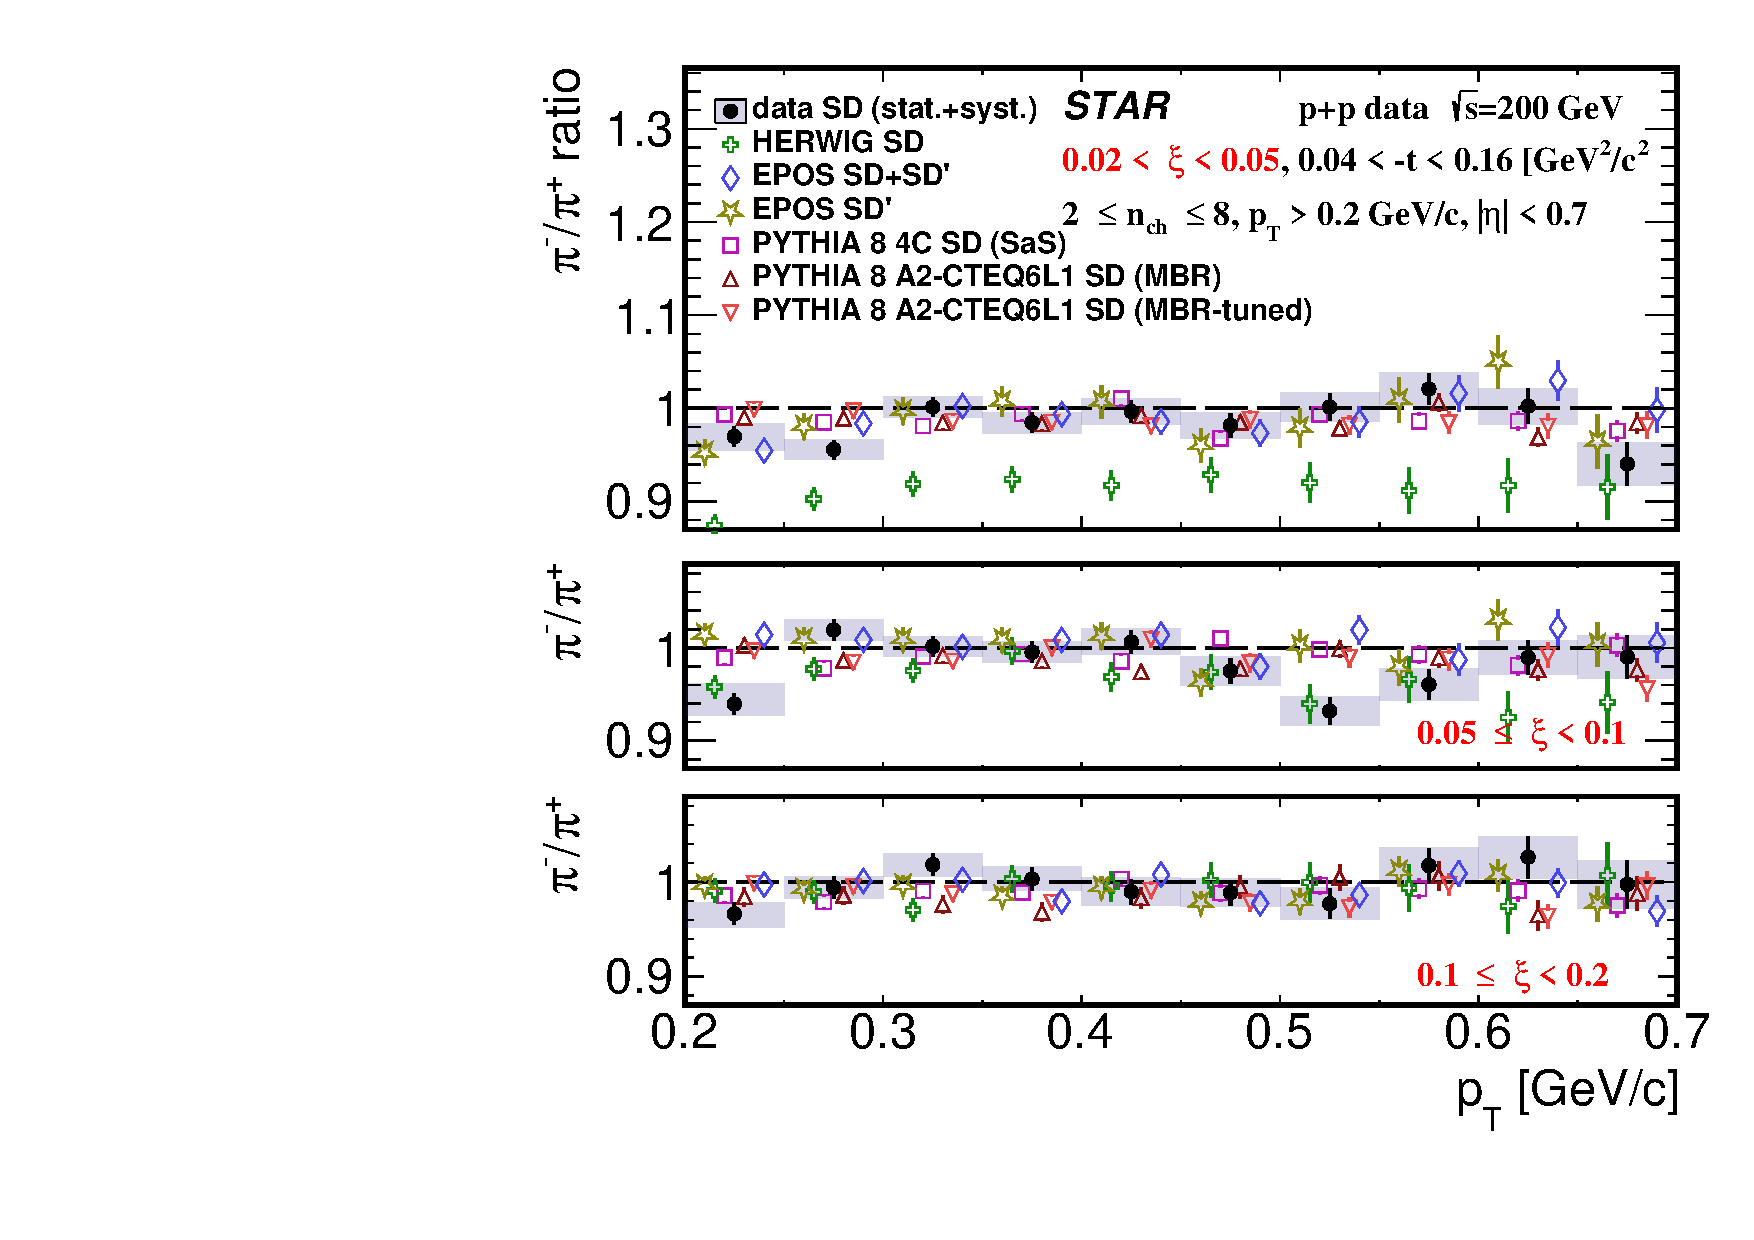
\includegraphics[width=.99\textwidth,page=1]{chapters/chrgSTAR/img/results/particleRatio_prt_0.pdf}
	%
	\caption{Ratio of production yields of $\pi^-/\pi^+$ as a function of $p_\textrm{T}$ shown separately for the~three ranges of $\xi$: (top) $0.02<\xi<0.05$, (middle) $0.05<\xi<0.1$, (bottom) $0.1<\xi<0.2$.}
	\label{fig:results_star_pion}
	
\end{figure}

Figure~\ref{fig:results_star_pion} shows the~ratio of production yields of $\pi^-/\pi^+$ as a function of $p_\textrm{T}$  separately for the~three ranges of $\xi$. Data in all three $\xi$ ranges are consistent with equal amounts of $\pi^+$ and $\pi^-$ with no significant $p_\textrm{T}$ dependence. Models agree with data (except HERWIG) predicting on average small deviation from unity by $\sim2\%$ what is smaller than data uncertainties. HERWIG in first two $\xi$ ranges predicts too large asymmetry between $\pi^+$ and $\pi^-$.

Figure~\ref{fig:results_star_kaon} shows the~ratio of production yields of $K^- / K^+$ as a function of $p_\textrm{T}$  separately for the~three ranges of $\xi$ . Data in all three $\xi$  ranges are consistent with equal amounts of $K^+$ and $K^-$ with no $p_\textrm{T}$ dependence. Models agree with data except HERWIG in the~first $\xi$  range predicting too large ratio of $K^-$ to $K^+$.
\begin{figure}[h!]
	\centering
	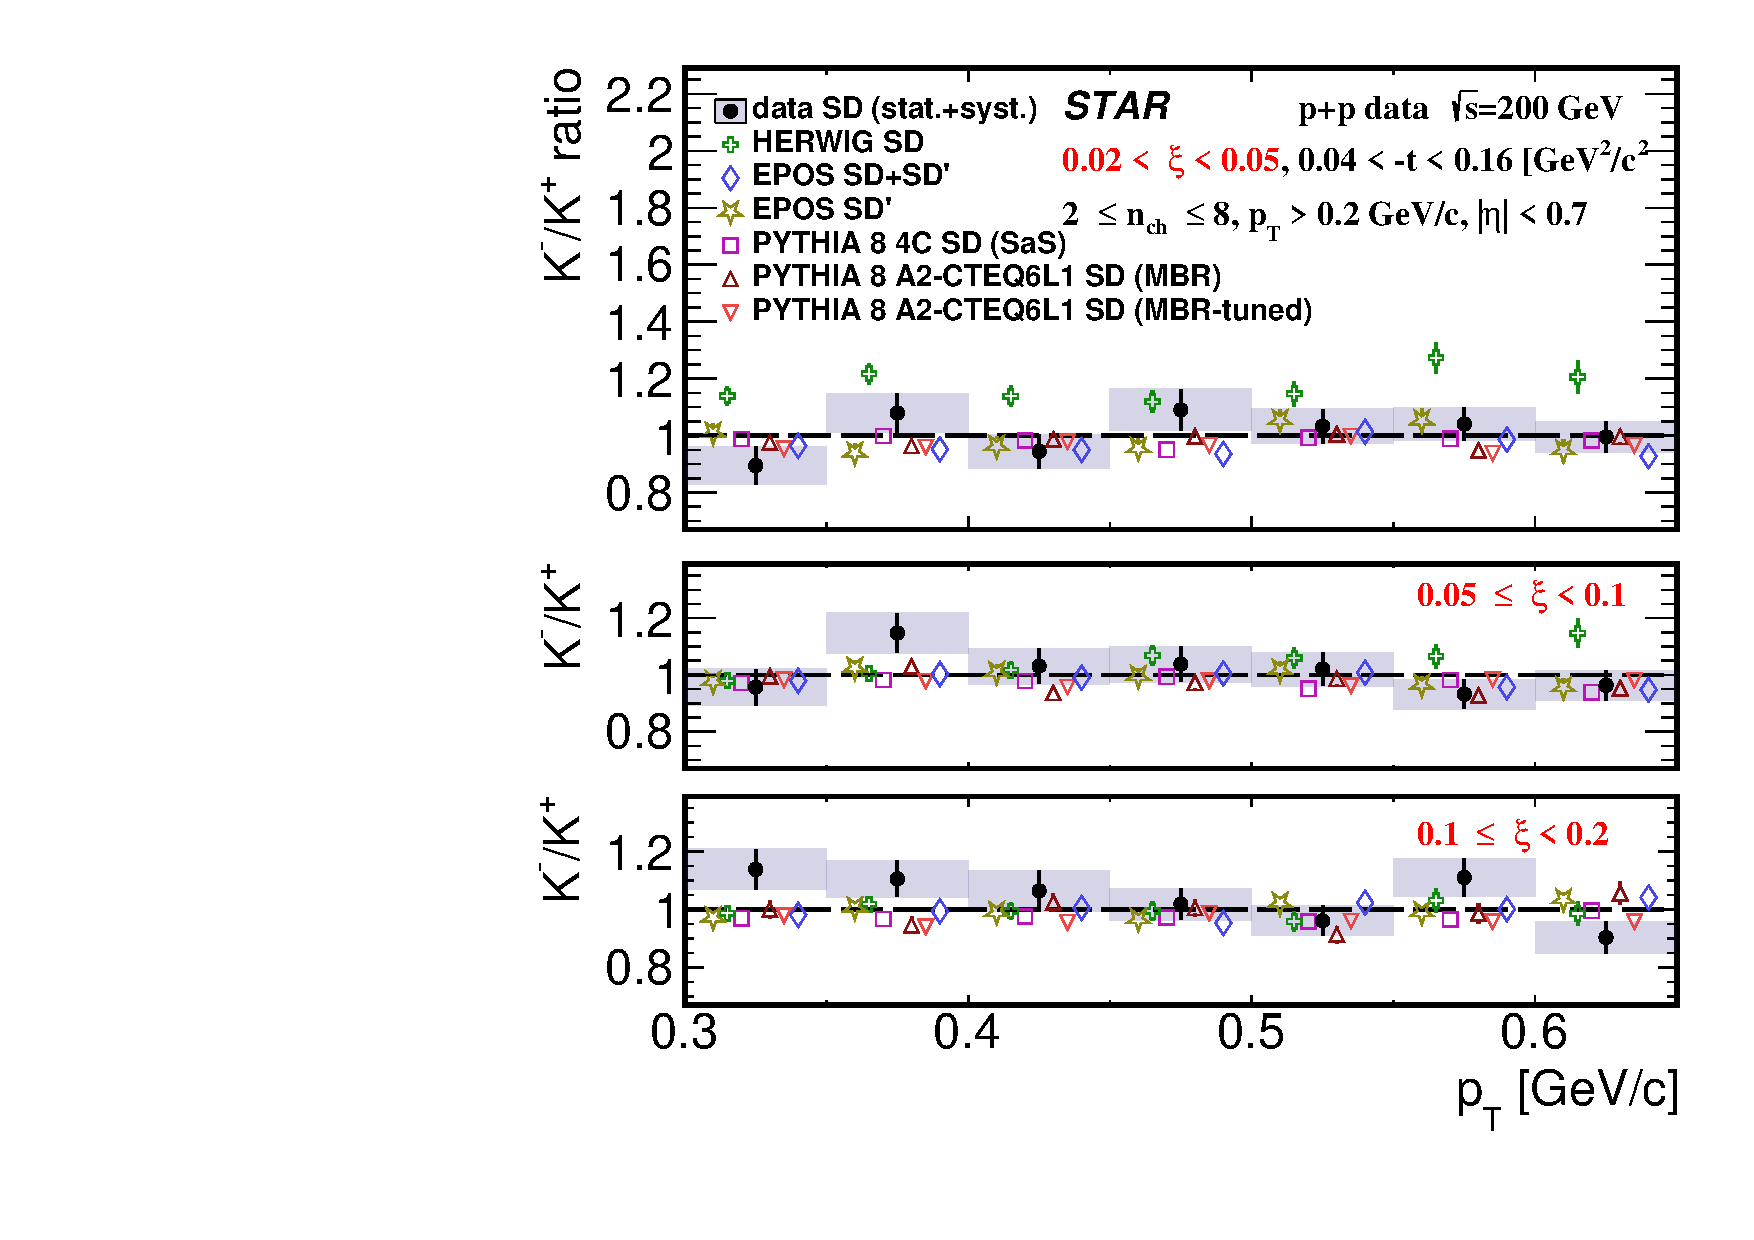
\includegraphics[width=.99\textwidth,page=1]{chapters/chrgSTAR/img/results/particleRatio_prt_1.pdf}
	%
	\caption{Ratio of production yields of $K^-/K^+$ as a function of $p_\textrm{T}$ shown separately for the~three ranges of $\xi$: (top) $0.02<\xi<0.05$, (middle) $0.05<\xi<0.1$, (bottom) $0.1<\xi<0.2$.}
	\label{fig:results_star_kaon}
	
\end{figure}

Figure~\ref{fig:results_star_proton} shows the~ratio of production yields of $\bar{p}/p$ as a function of $p_\textrm{T}$  separately for the~three ranges of $\xi$. Data in the~last two $\xi$ ranges are consistent with equal amounts of $p$ and $\bar{p}$ with no $p_\textrm{T}$ dependence. However, in the~first $\xi$ range at $p_\textrm{T}<0.7$~GeV/c data shows significant deviation from unity indicating a~significant transfer of the baryon number from the forward to the central region. PYTHIA8 and EPOS SD+SD$^\prime$ agree with data in the~last two $\xi$ ranges. In first $\xi$ range PYTHIA8 predicts small deviation from unity by $\sim5\%$ which is smaller than observed in data, whereas EPOS SD+SD$^\prime$ predicts an asymmetry between $\bar{p}$ and $p$ of $\sim30\%$  which is larger than observed in data except $p_\textrm{T}<0.5$~GeV/c. HERWIG predicts much larger baryon number transfer compared to data in first two $\xi$ ranges and shows consistency with data in last $\xi$ range. 

Figure~\ref{fig:results_mean_ratio_star} shows mean ratio of production yields of $\pi^-/\pi^+$, $K^-/K^+$ and $\bar{p}/p$ as a~function of  $\xi$.

\begin{figure}[h!]
	\centering
	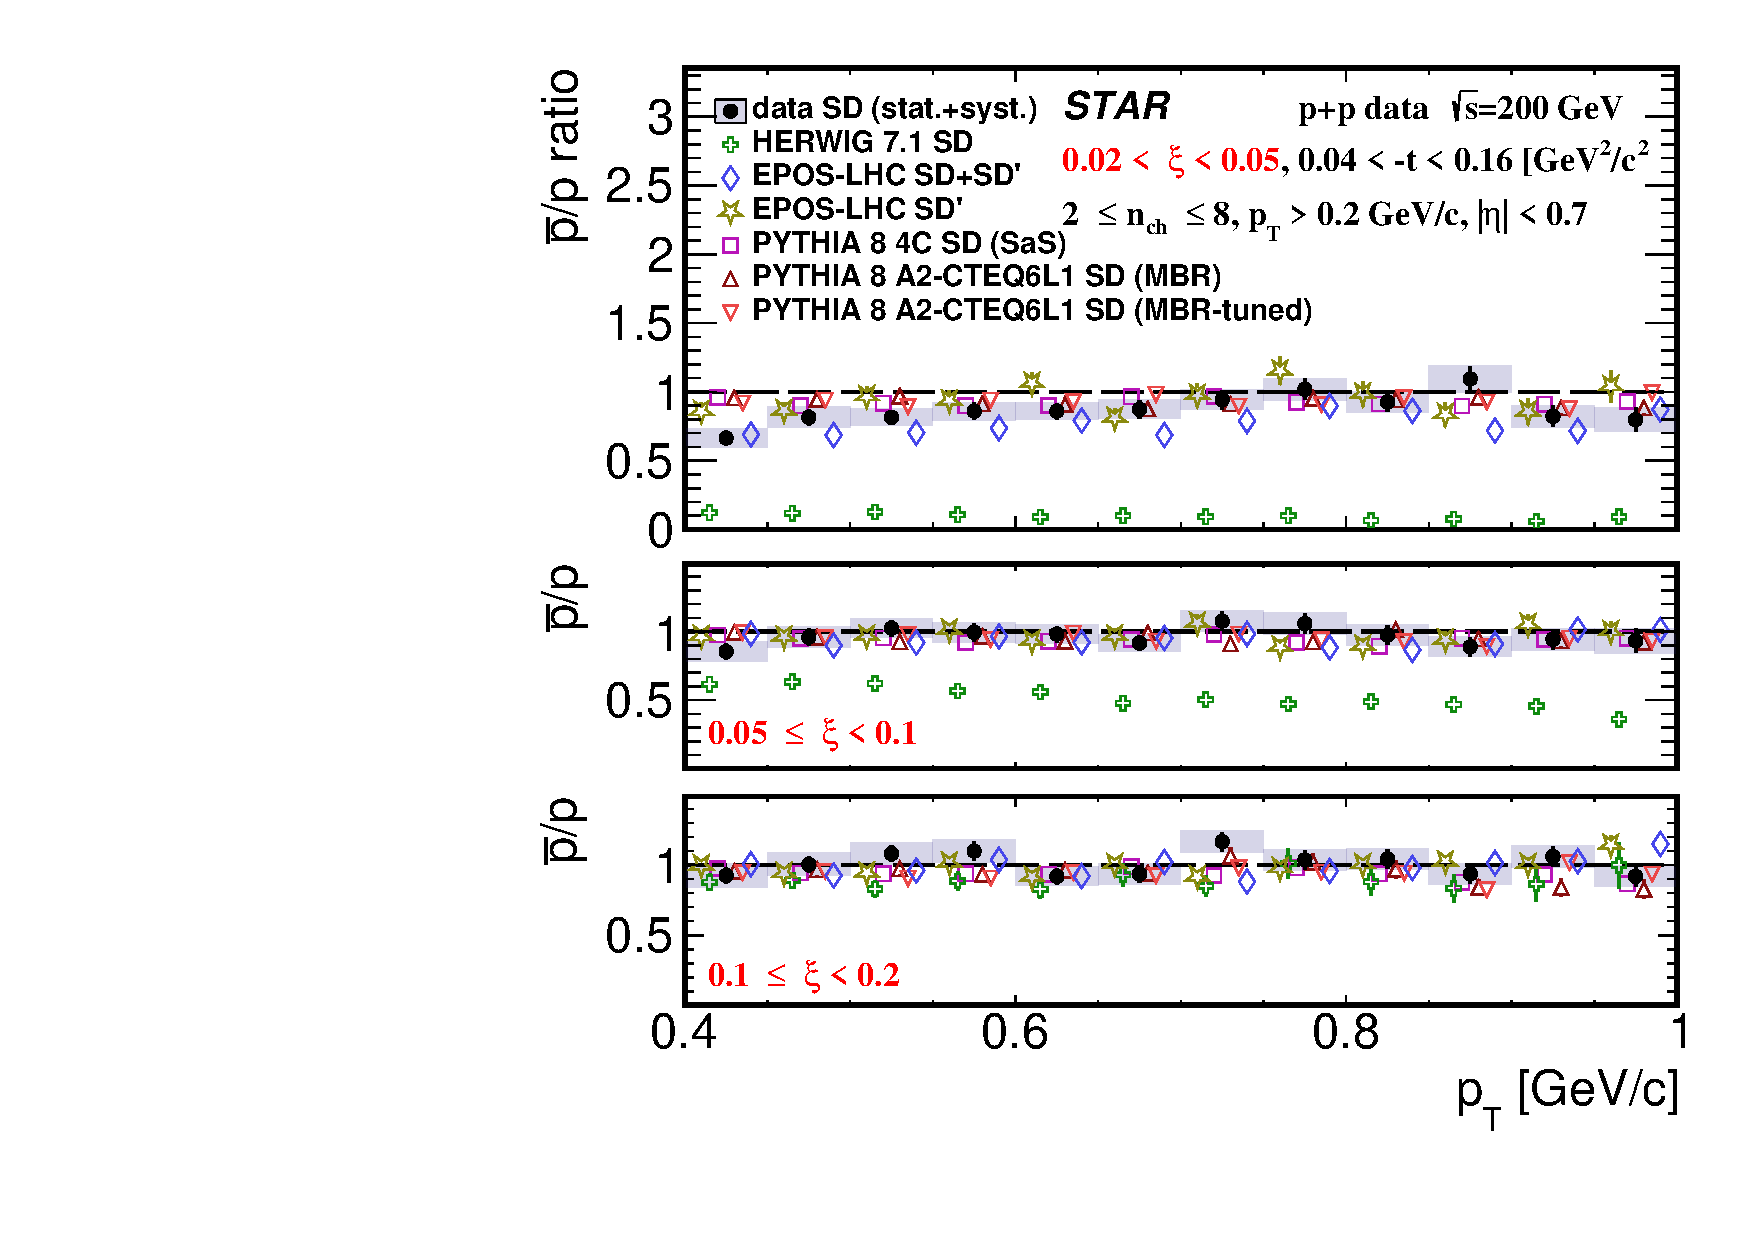
\includegraphics[width=.99\textwidth,page=1]{chapters/chrgSTAR/img/results/particleRatio_prt_2.pdf}
	%
	\caption{Ratio of production yields of $\bar{p}/p$ as a function of $p_\textrm{T}$ shown separately for the~three ranges of $\xi$: (top) $0.02<\xi<0.05$, (middle) $0.05<\xi<0.1$, (bottom) $0.1<\xi<0.2$.}
	\label{fig:results_star_proton}
	
\end{figure}

\begin{figure}[h!]
	\centering
	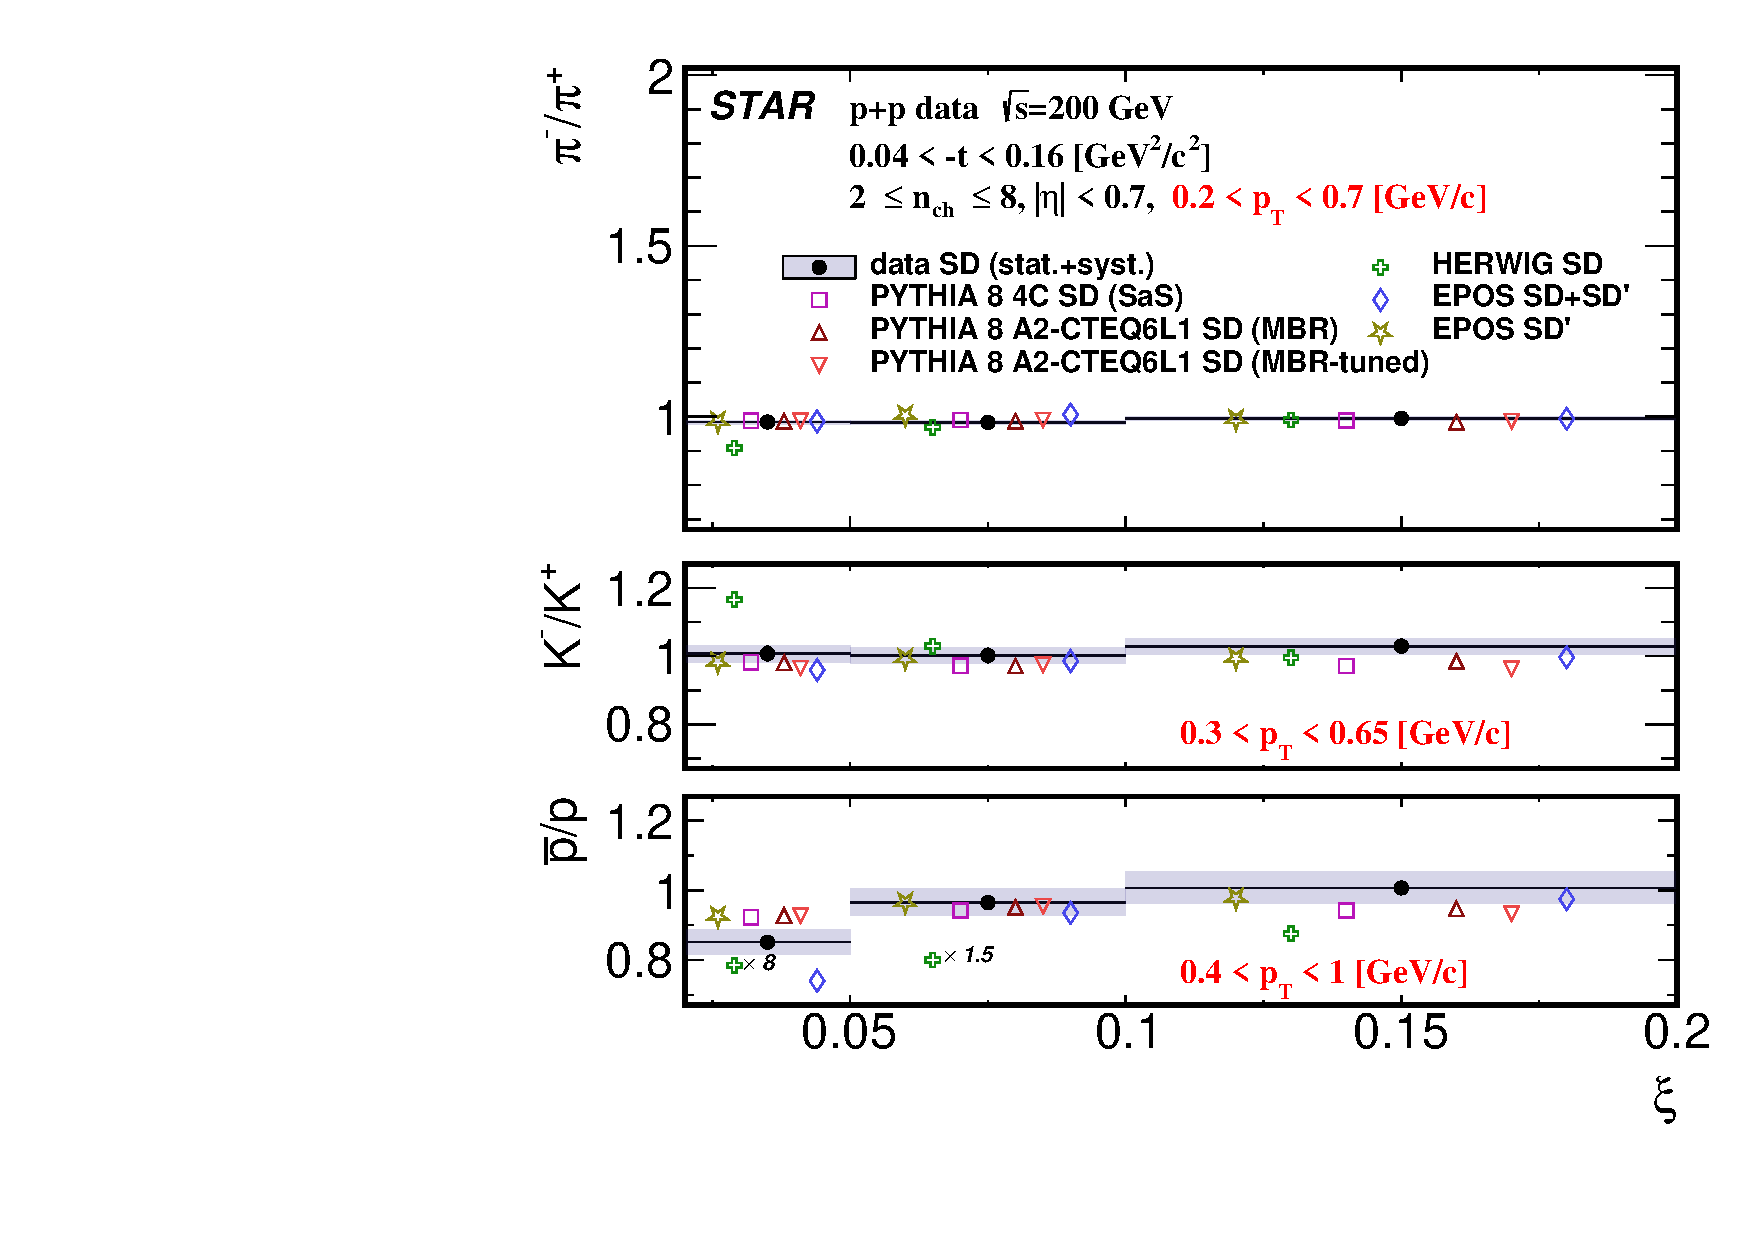
\includegraphics[width=.99\textwidth,page=1]{chapters/chrgSTAR/img/results/ratio_xi.pdf}
	%
	\caption{Ratio of production yields of $\pi^-/\pi^+$, $K^-/K^+$ and $\bar{p}/p$ as a~function of $\xi$. }
	\label{fig:results_mean_ratio_star}
	
\end{figure}